\documentclass[a4paper,10pt,conference,onecolumn]{IEEEtran}
\IEEEoverridecommandlockouts

% ── Packages ─────────────────────────────────────────────────────────────────
\usepackage{cite}
\usepackage{amsmath,amssymb,amsfonts}
\usepackage{algorithmic}
\usepackage{graphicx}
\usepackage{textcomp}
\usepackage{xcolor}
\usepackage{booktabs}
\usepackage{array}
\usepackage{tabularx}
\usepackage{multirow}
\usepackage{hyperref}
\usepackage{url}
\usepackage{balance}
\usepackage{float}
\usepackage{listings}
\usepackage{multicol}

\lstdefinestyle{leaksensecode}{
  basicstyle=\ttfamily\scriptsize,
  abovecaptionskip=0.6em,
  belowcaptionskip=0.9em,
  breaklines=true,
  breakatwhitespace=false,
  columns=fullflexible,
  keepspaces=true,
  numbers=left,
  numbersep=8pt,
  numberstyle=\tiny\color{gray},
  frame=single,
  rulecolor=\color{black!30},
  commentstyle=\color{green!40!black},
  keywordstyle=\color{blue!70!black},
  stringstyle=\color{red!60!black},
  showstringspaces=false,
  tabsize=2,
  literate=
    {—}{{--}}1
    {–}{{--}}1
    {─}{{-}}1
    {→}{{$\rightarrow$}}1
    {°}{{$^\circ$}}1
    {·}{{$\cdot$}}1
    {…}{{...}}3
}
\lstset{style=leaksensecode}

\lstdefinestyle{leaksensecodecompact}{
  style=leaksensecode,
  basicstyle=\ttfamily\tiny,
  aboveskip=0.25em,
  belowskip=0.25em,
  abovecaptionskip=0.2em,
  belowcaptionskip=0.2em,
  frame=none,
  numbers=left,
  numbersep=4pt,
  numberstyle=\fontsize{4.5}{5}\selectfont\color{gray},
  xleftmargin=1.6em,
  xrightmargin=0pt
}

\newcommand{\leaksenselisting}[4][]{%
  \refstepcounter{lstlisting}%
  \label{#3}%
  \begin{center}
    {\small Listing~\thelstlisting. #2}
  \end{center}
  \vspace{0.45em}
  \lstinputlisting[#1]{#4}
}

\newcommand{\leaksensecompactlisting}[4][]{%
  \refstepcounter{lstlisting}%
  \label{#3}%
  \noindent{\footnotesize\textbf{Listing~\thelstlisting. #2}}\par
  \vspace{0.15em}
  \lstinputlisting[#1]{#4}
}

\hypersetup{
  colorlinks=true,
  linkcolor=black,
  citecolor=black,
  urlcolor=blue,
  hypertexnames=false
}

% ── Metadata ─────────────────────────────────────────────────────────────────
\def\BibTeX{{\rm B\kern-.05em{\sc i\kern-.025em b}\kern-.08em
    T\kern-.1667em\lower.7ex\hbox{E}\kern-.125emX}}
\renewcommand\IEEEkeywordsname{Keywords}

\begin{document}

% ════════════════════════════════════════════════════════════════════════════
% TITLE
% ════════════════════════════════════════════════════════════════════════════
\title{LeakSense -- Smart LPG Gas Leakage Detection and\\Automatic Safety System}

\author{
  CITS5506 The Internet of Things\\
The University of Western Australia, Australia\\
Semester 1, 2026\\

\\

Group 27
\\
\\
  1\textsuperscript{st} Yuxuan Xi, 24319908@student.uwa.edu.au\\
  2\textsuperscript{nd} Yiming Zhao, 24139958@student.uwa.edu.au;\\
  3\textsuperscript{rd} Sahil Pankajbhai Patel, 24562775@student.uwa.edu.au;\\
  4\textsuperscript{th} Sohaib Ahmed Khan, 24756957@student.uwa.edu.au\\
}

\maketitle
% ════════════════════════════════════════════════════════════════════════════
% ABSTRACT
% ════════════════════════════════════════════════════════════════════════════
\noindent\rule{\linewidth}{0.4pt}
\vspace{0.6em}

\begin{abstract}
Residential LPG leakage is a serious household safety problem because
accumulated gas can cause fire, explosion, and health hazards, yet affordable
detectors typically provide only local alarms without physical mitigation or
remote monitoring. This report presents LeakSense, a low-cost Internet of
Things system that detects LPG risk, responds locally, and provides
real-time cloud visibility. The system was developed using an iterative
development method and integrates an ESP32 microcontroller, a MEMS gas sensor,
a BME280 atmospheric sensor, relay-driven actuators, Firebase Realtime
Database, and a browser dashboard. The firmware samples gas voltage every two
seconds and classifies readings into Safe, Warning, Danger, and Extreme
states, escalating Warning to Danger when abnormal temperature rise or high
absolute temperature indicates additional thermal risk. Local actuators
operate independently of network connectivity, while Firebase uploads support
live status, history logging, and browser notifications. Testing confirmed
correct state classification across all thresholds, actuator response within
the two-second polling interval, cloud-to-dashboard updates within three
seconds, successful push notifications, and continued local safety operation
during Wi-Fi interruption. LeakSense cost approximately \$94~AUD. Key
limitations are the small-scale fan, the absence of an automatic gas
shutoff valve, and empirically determined voltage thresholds that require
formal calibration against certified reference gas for production deployment.
\end{abstract}

\begin{IEEEkeywords}
Internet of Things; LPG gas detection; ESP32; Firebase; dual-sensor
escalation; residential safety; web dashboard
\end{IEEEkeywords}

\vspace{0.4em}
\noindent\rule{\linewidth}{0.4pt}
\vspace{0.8em}

% ════════════════════════════════════════════════════════════════════════════
% I. PROBLEM STATEMENT
% ════════════════════════════════════════════════════════════════════════════
\section{Problem Statement}

LPG is used in over two million Australian households for cooking, heating,
and hot water systems \cite{gasEnergy2020}. In its natural state, LPG is
odourless and can accumulate to dangerous concentrations before occupants
become aware of a leak. According to Fire and Rescue NSW, gas-related
incidents account for a significant proportion of residential fire call-outs
each year \cite{fireRescue2023}.

Existing residential gas detection solutions fail to address the full scope of
this safety problem. Basic standalone detectors produce only a local audible
alarm, which is ineffective when occupants are asleep, absent, or
hearing-impaired, and do not initiate any physical hazard mitigation. Smart
consumer detectors provide mobile push notifications but remain proprietary,
do not control physical ventilation, and do not expose sensor data for custom
analysis. Research-grade IoT prototypes have demonstrated remote alerting but
typically use analog sensors without environmental compensation, rely on
single-sensor detection, and lack multi-threshold response logic and
cloud-connected dashboards \cite{islam2020}. Industrial detection systems
provide certified shutoff valve integration and high measurement accuracy but
are prohibitively expensive for residential installation.

A critical and unaddressed limitation across all affordable solutions is the
absence of multi-factor escalation. Gas leakage in combination with a sudden
rise in ambient temperature --- which may indicate an ignition or fire risk
--- is not modelled in any existing consumer product. The central problem is
therefore the absence of an affordable, integrated residential solution that
combines: continuous gas voltage monitoring, graduated multi-threshold
response with thermal escalation, automatic physical hazard mitigation, and
remote cloud-based monitoring with historical data logging. LeakSense is
designed specifically to fill this gap.

% ════════════════════════════════════════════════════════════════════════════
% II. INTRODUCTION
% ════════════════════════════════════════════════════════════════════════════
\section{Introduction}

The Internet of Things enables physical sensor systems to communicate with
cloud infrastructure and user-facing applications, creating safety systems
that respond both locally and remotely. LeakSense applies this IoT
architecture to the practically important problem of residential LPG gas
leakage detection, extending prior single-sensor approaches with a
dual-sensor escalation model that integrates gas concentration voltage with
ambient temperature readings.

Prior work in this area falls into four broad categories. First, passive
standalone detectors provide local alarms but no remote awareness or physical
response. Second, smart consumer products add cloud notification but maintain
proprietary data ecosystems that prevent custom integration. Third, academic
IoT prototypes demonstrate cloud-connected gas detection using commodity
microcontrollers but typically rely on single analog MQ-series sensors without
environmental compensation \cite{islam2020}\cite{sarkar2024}. Fourth,
industrial systems provide the most complete safety response but at a scale
and cost entirely unsuitable for residential use. A consistent limitation
across affordable solutions is the absence of automatic ventilation control,
thermal escalation logic, and real-time web-based monitoring with historical
trend data \cite{saeed2018}.

This report describes the design, implementation, and testing of LeakSense ---
a system that addresses the identified gaps using a FireBeetle ESP32-E
microcontroller, a SEN0565 MEMS analog gas sensor, a BME280 atmospheric
sensor, relay-controlled actuators, Firebase Realtime Database via HTTPS REST,
and a plain HTML/CSS/JavaScript web dashboard. The system was designed using
an iterative prototyping methodology. Success was defined as correct state
classification across all thresholds, actuator response within two seconds,
end-to-end cloud-to-dashboard latency within three seconds, and continued local
safety operation during Wi-Fi interruption.

The remainder of this report is structured as follows. Section~\ref{sec:arch}
describes the system architecture and hardware design.
Section~\ref{sec:firmware} presents the firmware implementation including
thermal escalation logic. Section~\ref{sec:dashboard} describes the web
dashboard and cloud architecture. Section~\ref{sec:testing} presents testing
methodology and results. Section~\ref{sec:limitations} discusses limitations
and future work. Section~VIII presents the project cost. Section~\ref{sec:conclusion}
concludes the report. Section~\ref{sec:howto} provides instructions for
hardware setup, firmware installation, Firebase configuration, and dashboard
operation. The references follow the How-To Guide, and the appendices provide
the code function explanations and source code listings.

% ════════════════════════════════════════════════════════════════════════════
% III. SYSTEM ARCHITECTURE
% ════════════════════════════════════════════════════════════════════════════
\section{System Architecture}
\label{sec:arch}

\subsection{Overview}

LeakSense is structured around five IoT layers: sensing, computing,
actuation, cloud communication, and user interface. The block diagram in
Fig.~\ref{fig:arch} illustrates the five subsystems, their data flows, and
their interconnections. Two distinct data paths exist: a local safety path
from sensing through processing to actuation that operates continuously
regardless of network availability, and a cloud path from processing through
Firebase to the dashboard that operates on a best-effort basis.

The ESP32 is the central integration point. It polls the gas sensor and
BME280 every two seconds, applies a two-pass state classification algorithm
(voltage thresholds followed by a thermal escalation check), drives all local
actuators independently of network availability, and publishes data to
Firebase every two seconds for the live dashboard and every five minutes for
historical records.

\begin{figure}[H]
  \centering
  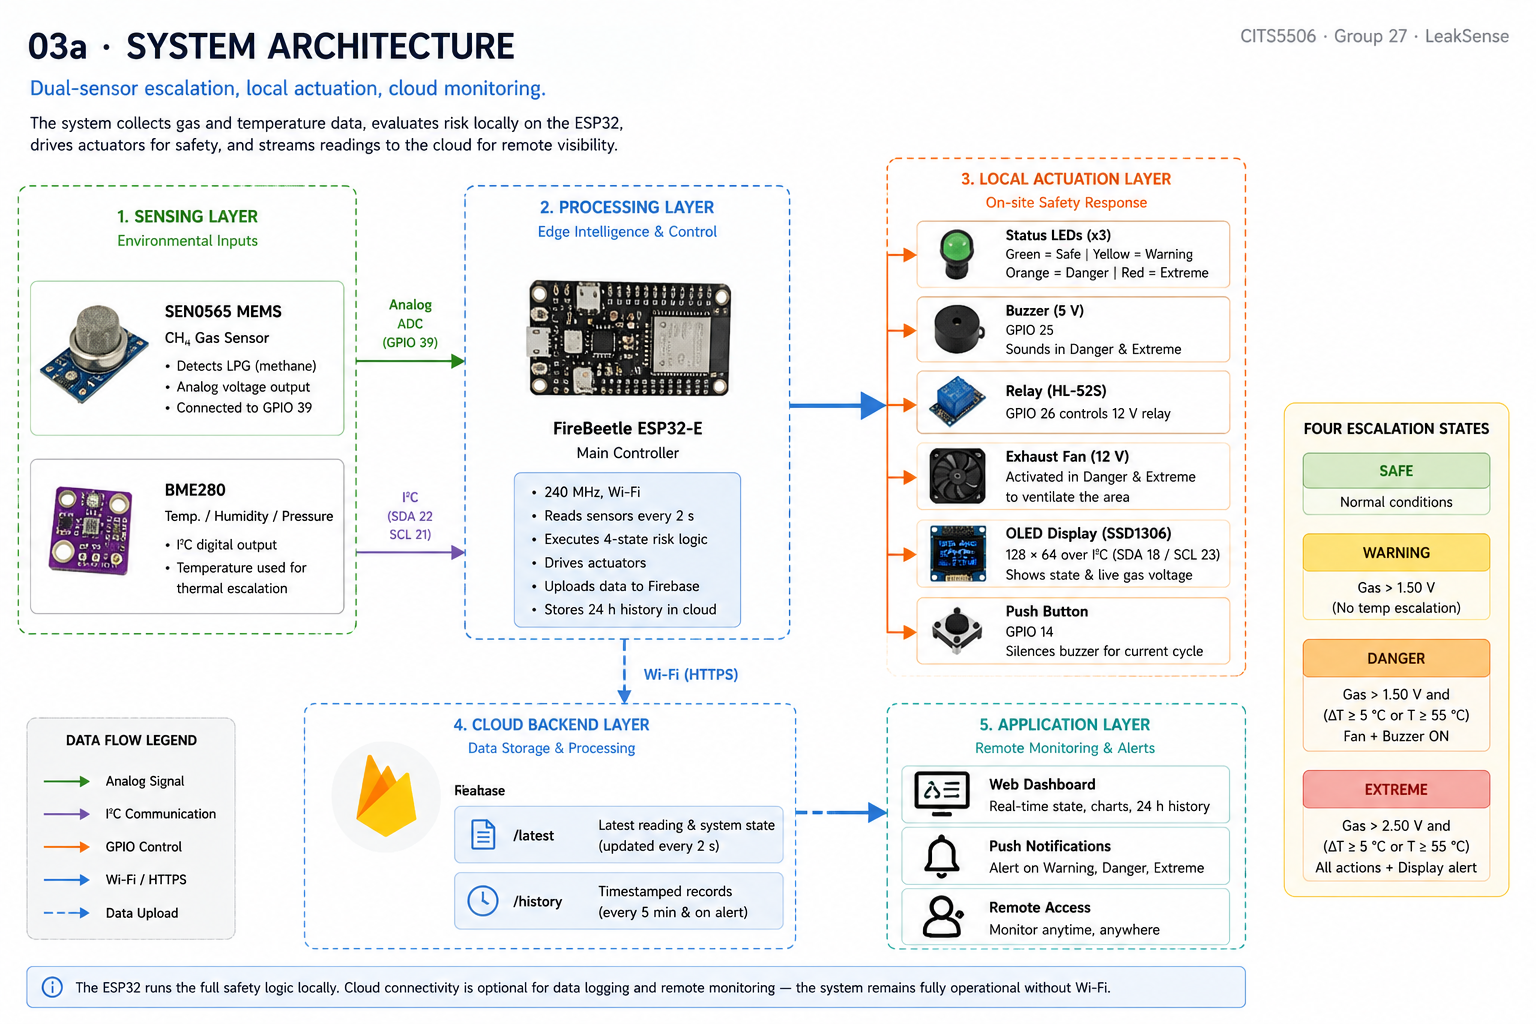
\includegraphics[width=0.9\linewidth]{system_architecture.png}
  \caption{LeakSense system block diagram showing all five IoT layers and
  their interconnections. (REST = Representational State Transfer;
  HTTPS = Hypertext Transfer Protocol Secure; LED = light-emitting diode;
  OLED = organic light-emitting diode.)}
  \label{fig:arch}
\end{figure}

\subsection{Component Overview}

Table~\ref{tab:components} lists all hardware components used in the
LeakSense system.

\begin{table}[H]
\centering
\caption{LeakSense hardware components and GPIO assignments.}
\label{tab:components}
\renewcommand{\arraystretch}{1.2}
\setlength{\tabcolsep}{6pt}
\begin{tabularx}{\linewidth}{
  >{\raggedright\arraybackslash}p{3.4cm}
  >{\raggedright\arraybackslash}X
  >{\centering\arraybackslash}p{1.7cm}
  >{\centering\arraybackslash}p{1.7cm}}
\toprule
\textbf{Component} & \textbf{Purpose} & \textbf{GPIO} & \textbf{Bus} \\
\midrule
FireBeetle ESP32-E & Central MCU --- Wi-Fi, I2C, GPIO, 240\,MHz dual-core
  & --- & ---\\
SEN0565 MEMS CH4 & Analog gas voltage --- primary input & 39 & ADC\\
BME280 & Temp (escalation) + Humidity (display) & 22/21 & I2C-1 \\
OLED SSD1306 128$\times$64 & Local real-time status display & 18/23 & I2C-0
\\
HL-52S Relay & Controls exhaust fan & 26 & GPIO\\
12\,V Exhaust Fan & Ventilation via relay & (relay) & --- \\
5\,V Buzzer & Audible alarm --- 10\,s cycle & 25 & GPIO\\
Green LED & Safe state indicator & 17 & GPIO\\
Yellow LED & Warning state indicator & 16 & GPIO\\
Red LED & Danger/Extreme indicator & 4 & GPIO\\
Push Button & Silences current buzzer cycle & 14 & GPIO\\

\bottomrule
\end{tabularx}
\end{table}

\subsection{Component Descriptions}

\subsubsection{FireBeetle ESP32-E}
The FireBeetle ESP32-E was selected because it integrates Wi-Fi, two I2C
buses, ADC-capable GPIO, and a dual-core 240\,MHz processor on one compact
board. It is fully compatible with PlatformIO and the Arduino framework,
which reduces firmware development time. The built-in Wi-Fi module enables
direct HTTPS REST communication with Firebase Realtime Database without an
additional networking component \cite{espressif2026}.The FireBeetle ESP32-E board is shown in
Fig.~\ref{fig:esp32}.

\begin{figure}[H]
  \centering
  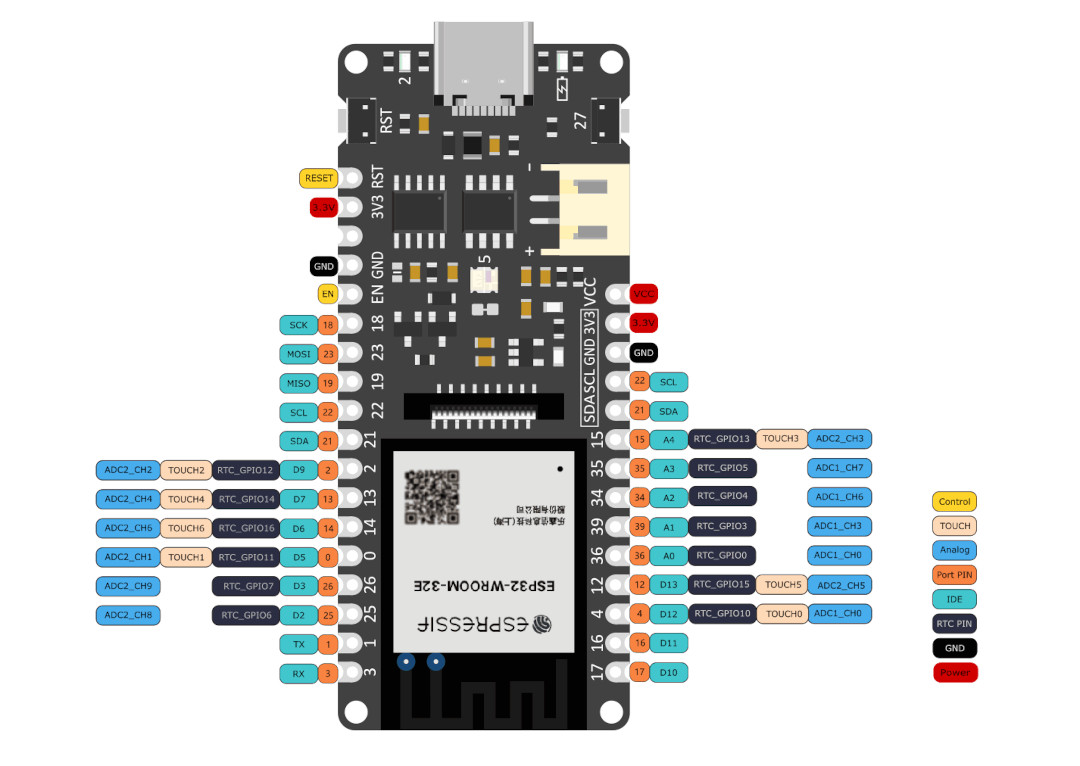
\includegraphics[width=0.70\linewidth]{firebeatle_ESP32-E.jpg}
  \caption{FireBeetle ESP32-E Microcontroller serving as the central processing unit, responsible for sensor polling, state classification, actuator control, and cloud communication.}
  \label{fig:esp32}
\end{figure}

\subsubsection{SEN0565 MEMS CH4 Gas Sensor}
The SEN0565 Fermion MEMS CH4 sensor was selected as the primary gas
detection input. The sensor outputs an analog voltage on GPIO~39 that rises
with increasing gas concentration, without requiring manual Rs/R0 resistance
ratio conversion or sensitivity curve calculation. DFRobot documentation
confirms the sensor is intended for qualitative measurement only and does not
output calibrated concentration values in parts per million
\cite{sen0565wiki}. The sensor requires a warm-up period of at least five
minutes before readings are stable, and 24 hours if it has been unused for
an extended period \cite{sen0565warmup}.

Because no manufacturer-certified LPG-to-voltage mapping exists for this
sensor, voltage thresholds were determined empirically by observing serial
monitor output during controlled lighter-gas exposure in a laboratory
environment. The resulting thresholds --- 1.60\,V for Warning and 1.90\,V
for Danger --- are empirical calibration constants. For a production safety
system, formal calibration against certified LPG reference gas or a known
percentage lower-explosive-limit (LEL) standard would be required. The OSHA
chemical data for LPG states that the LEL for propane is approximately 2.1\%
by volume and 1.9\% for butane \cite{osha2024}, which would serve as the
reference concentration targets for proper calibration.The SEN0565 sensor module is shown in Fig.~\ref{fig:sen0565}.

\begin{figure}[H]
  \centering
  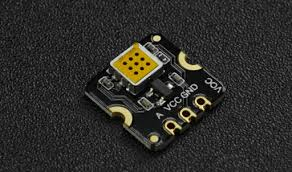
\includegraphics[width=0.30\linewidth]{SEN0565_MEMS CH4_Sensor.jpeg}
  \caption{SEN0565 MEMS CH4 Sensor providing an analog voltage output proportional to gas concentration, used as the primary input for state classification.}
  \label{fig:sen0565}
\end{figure}

\subsubsection{BME280 Atmospheric Sensor}
The BME280 provides ambient temperature and humidity measurements over I2C
on a dedicated bus (SDA GPIO~22, SCL GPIO~21) \cite{bme280}. Temperature serves as a
secondary escalation input: if the temperature rises 5\,$^{\circ}$C or more
between consecutive two-second readings, or reaches 55\,$^{\circ}$C
absolute, and the gas state is already Warning, the system escalates
immediately to Danger and records \texttt{thermal\_risk: true} in the
Firebase payload. Humidity is displayed on the dashboard for environmental
context and has no effect on the safety state. This dual-sensor approach is
supported by Wu~et~al., who demonstrated that combining gas and temperature
measurements significantly reduces false positive alarm rates compared to
single-sensor designs \cite{wu2021}.The BME280 module is shown in Fig.~\ref{fig:bme280}.

\begin{figure}[H]
  \centering
  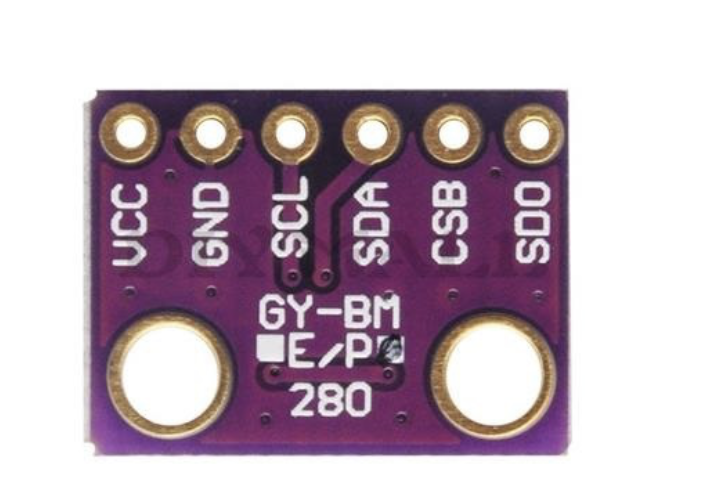
\includegraphics[width=0.30\linewidth]{BME280_atmospheric.png}
  \caption{BME280 Atmospheric Sensor providing temperature and humidity readings for thermal escalation and dashboard display.}
  \label{fig:bme280}
\end{figure}

\subsubsection{OLED Display SSD1306}
The SSD1306 0.96-inch I2C OLED display provides the local visual interface
for the device. It was selected because it operates from 3.3\,V logic and
power, which is directly compatible with the ESP32 without level-shifting,
and because its small footprint suits a compact enclosure
\cite{ssd1306core}. The display is connected to a dedicated I2C bus
(TwoWire~0) on SDA GPIO~18 and SCL GPIO~23 at address 0x3C, separated from
the BME280 bus to avoid address contention.

During operation the display shows the current temperature, humidity, gas
voltage, baseline voltage, classified state (Safe, Warning, or Danger), and
the on/off status of the fan and buzzer, as drawn by the
\texttt{drawStatusScreen()} routine in Section~\ref{sec:firmware}. This
makes the device usable as a standalone unit during demonstrations without
opening the web dashboard, and it accelerated firmware debugging during
development because sensor readings and state transitions could be observed
directly on the device. The OLED module is shown in Fig.~\ref{fig:oled}.

\begin{figure}[H]
  \centering
  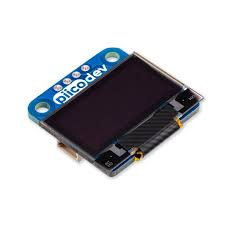
\includegraphics[width=0.30\linewidth]{OLED_SSD1306.jpeg}
  \caption{0.96-inch SSD1306 I2C OLED display providing local status output, showing live temperature, humidity, gas voltage, and classified safety state.}
  \label{fig:oled}
\end{figure}

\subsubsection{Buzzer and LED Indicators}
The buzzer provides the audible local alarm when the system enters the
Danger state. A Gravity digital buzzer module was selected because it is
driven directly from a single GPIO line --- it accepts a HIGH/LOW logic
signal from the ESP32 and requires no PWM generation or external driver
circuitry \cite{gravitybuzzer}. It is connected to GPIO~25 and operates on
the ten-second on/off cycle described in Section~\ref{sec:firmware}.

Three through-hole LEDs provide additional visual status indication
independent of the OLED: green (GPIO~17) for the Safe state, yellow
(GPIO~16) for Warning, and red (GPIO~4) for Danger and Extreme. Each LED is
wired through a 270\,$\Omega$ current-limiting resistor to ground to keep
forward current within the safe operating range for standard 5\,mm LEDs at
3.3\,V logic level. The three-colour scheme allows the system state to be
identified at a glance from across a room, complementing the more detailed
OLED readout. The buzzer module is shown in Fig.~\ref{fig:buzzer}.

\begin{figure}[H]
  \centering
  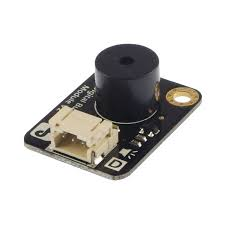
\includegraphics[width=0.30\linewidth]{Gravity_Buzzer.jpeg}
  \caption{Gravity digital buzzer module providing the audible alarm during Danger and Extreme states, driven from GPIO~25.}
  \label{fig:buzzer}
\end{figure}

\subsubsection{Relay Module and Exhaust Fan}
The HL-52S 5\,V single-channel relay module provides the switching interface
between the ESP32 and the exhaust fan. The ESP32 cannot directly drive
motor-class loads from its GPIO pins, so the relay isolates the
microcontroller from the fan's switching transients while allowing a
logic-level signal to control the higher-current path. The HL-52S is rated
to switch up to 10\,A at 28\,VDC and draws approximately 60\,mA at 5\,V
during activation, well within the project power budget
\cite{hl52srelay}. It is driven from GPIO~26 with active-low polarity
matching the module design.

The Delta 5\,V DC frameless exhaust fan (40\,mm, $\sim$0.1\,A,
$\sim$3150\,RPM) is the project's physical mitigation device
\cite{deltafan}. When the gas concentration crosses the Danger threshold,
the relay closes the fan supply circuit and the fan disperses accumulated
gas in the monitored space. This is the design choice that elevates
LeakSense from a passive alarm system to an active safety system --- the
fan provides immediate hazard mitigation without waiting for occupant
intervention. The 40\,mm form factor is appropriate for laboratory
demonstration; a production deployment would substitute a mains-rated
exhaust fan or integrate with existing kitchen ventilation, as discussed
in Section~\ref{sec:limitations}. The fan is shown in Fig.~\ref{fig:fan}.

\begin{figure}[H]
  \centering
  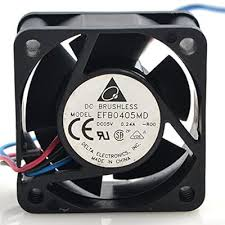
\includegraphics[width=0.30\linewidth]{Delta_5V_Fan.jpeg}
  \caption{Delta 5\,V DC 40\,mm frameless exhaust fan, switched via the HL-52S relay on GPIO~26 to disperse accumulated gas during Danger and Extreme states.}
  \label{fig:fan}
\end{figure}

\subsubsection{Supporting Assembly Components}
The remaining components support wiring, assembly, and stable testing of
LeakSense. An 830 tie-point solderless breadboard with dual isolated
power rails was used as the development platform because it provides
sufficient connection density for the seven sensor and actuator modules
without requiring soldered interconnects \cite{breadboard830}.
Male-to-male and male-to-female jumper wires route signals between the
ESP32 and the sensor and output modules, with male-to-female ends used for
the sensor and OLED headers that expose female pin sockets. A USB-A to
USB-C cable supplies 5\,V power to the FireBeetle ESP32-E and provides the
serial programming and debugging interface to the development host. A
push button on GPIO~14, configured with the ESP32 internal pull-up
resistor, allows the operator to silence the current buzzer cycle as
described in Section~\ref{sec:firmware}. A small project enclosure was
used during testing to simulate a partially enclosed residential space in
which leaked gas can accumulate to a detectable concentration around the
SEN0565 sensing element.
\\
\subsection{Circuit Wiring}

Two separate I2C buses are used. Bus~0 (TwoWire~0) operates on SDA GPIO~18
and SCL GPIO~23, serving the OLED SSD1306 display at I2C address 0x3C. Bus~1
(TwoWire~1) operates on SDA GPIO~22 and SCL GPIO~21, serving the BME280 at
address 0x76 or 0x77. This separation prevents address conflicts. The
SEN0565 analog output connects to GPIO~39, configured as a 12-bit ADC input
with 11\,dB attenuation for a full 0--3.3\,V measurement range.

The relay module is driven from GPIO~26 (active-low, matching the HL-52S
module polarity) and switches the exhaust fan's 12\,V supply rail. The
buzzer is driven from GPIO~25. Green, yellow, and red LEDs connect through
270\,$\Omega$ current-limiting resistors to GPIO~17, GPIO~16, and GPIO~4
respectively. The push button connects GPIO~14 to ground with the ESP32
internal pull-up resistor enabled.

Fig.~\ref{fig:schematic} shows the complete electrical setup used for the
LeakSense. It identifies the ESP32 GPIO assignments, the two separate I2C
buses, the SEN0565 analog input path, the LED indicator outputs, the alarm
button input, and the relay-controlled fan and buzzer structure. This diagram
therefore acts as the wiring reference for how the hardware subsystems are
connected to the microcontroller.

\begin{figure}[H]
  \centering
  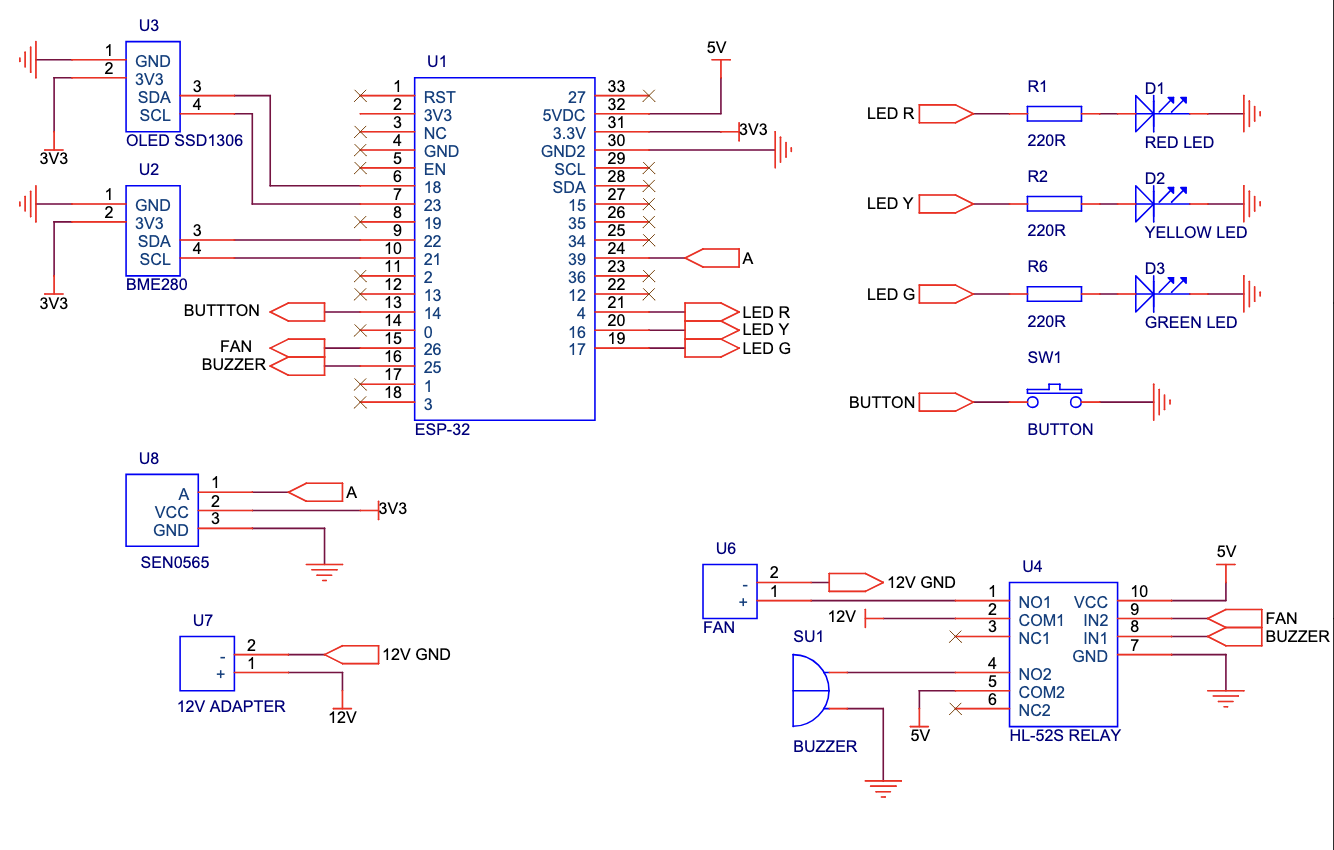
\includegraphics[width=0.95\linewidth]{system_diagram.png}
  \caption{LeakSense electronic schematic showing the ESP32 pin assignments,
  dual I2C sensor buses, SEN0565 analog input, LED indicators, push button,
  relay module, buzzer, fan, and 12\,V/5\,V power connections.}
  \label{fig:schematic}
\end{figure}

Fig.~\ref{fig:circuit} is the physical representation of the same circuit on
the breadboard. It shows how the schematic connections were implemented in the
system, including the ESP32-E placement, sensor modules, OLED display,
relay module, fan, buzzer, LEDs, and jumper-wire routing used during testing.

\begin{figure}[H]
  \centering
  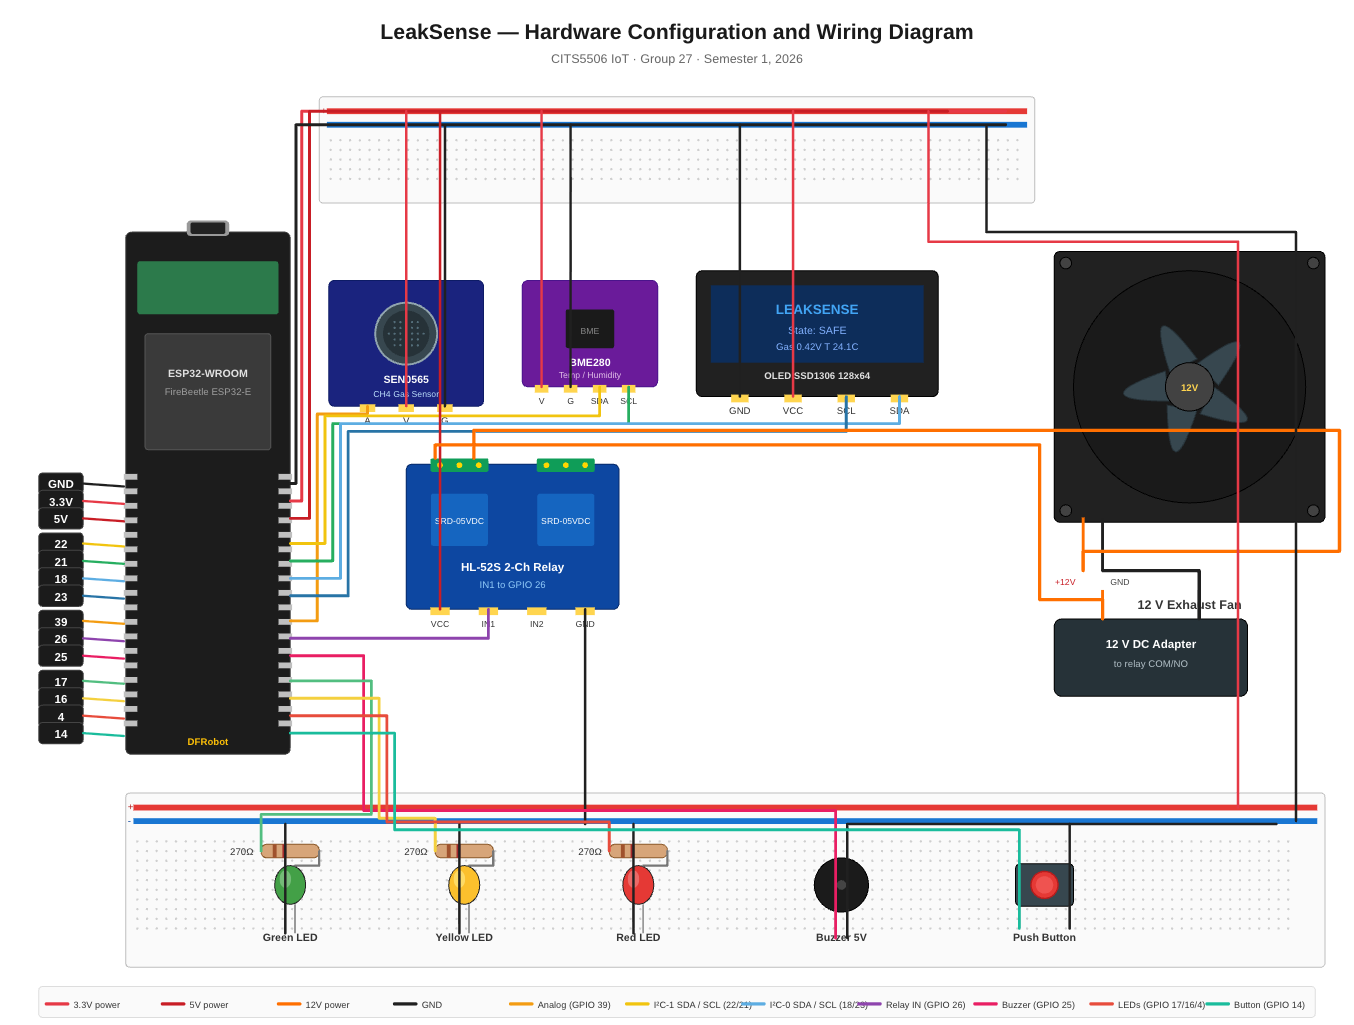
\includegraphics[width=0.9\linewidth]{circuit_wiring.png}
  \caption{LeakSense breadboard circuit showing the ESP32-E,
  SEN0565, BME280, OLED, relay module, fan, buzzer, and LEDs.}
  \label{fig:circuit}
\end{figure}

% ════════════════════════════════════════════════════════════════════════════
% IV. FIRMWARE IMPLEMENTATION
% ════════════════════════════════════════════════════════════════════════════
\section{Firmware Implementation}
\label{sec:firmware}

\subsection{Design Approach}

The firmware was developed in PlatformIO using the Arduino framework and an
iterative prototyping methodology. Each subsystem --- I2C sensors, state
machine, thermal escalation, and Firebase REST publishing --- was verified
independently before the next dependency was added. This approach ensured
working baselines at each stage and minimised debugging complexity during
integration.

\subsection{Boot Sequence}

On power-up the firmware executes six initialisation steps:
\begin{enumerate}
  \item All GPIO pins are set to safe defaults: green LED on, all alarm
        actuators off, relay off.
  \item A relay self-test fires for 500\,ms to confirm hardware continuity.
  \item I2C bus~0 is initialised and scanned, followed by OLED display
        initialisation at address 0x3C.
  \item I2C bus~1 is initialised and scanned, followed by BME280
        initialisation at address 0x76/0x77.
  \item The SEN0565 ADC input is configured on GPIO~39 with 12-bit resolution
        and 11\,dB attenuation. A ten-second baseline period is enforced with
        a serial monitor warning to allow sensor pre-heating. The manufacturer
        recommends at least five minutes warm-up \cite{sen0565warmup}.
  \item Wi-Fi connection is attempted with a ten-second timeout, followed by
        Firebase initialisation if connected. If Wi-Fi fails, the system
        continues in offline mode with all local safety functions active.
\end{enumerate}

\subsection{State Classification}

State classification is a two-pass algorithm executed on every two-second
polling cycle. The first pass derives the base state from the gas sensor
voltage reading using fixed thresholds. The second pass applies the thermal
escalation check. The firmware defines three hardware states; Table~\ref{tab:states}
defines the complete state-to-action mapping including the Extreme dashboard
display label.

\begin{table}[H]
\centering
\caption{State machine: voltage thresholds, firmware states, dashboard
labels, and system responses.}
\label{tab:states}
\renewcommand{\arraystretch}{1.3}
\small
\setlength{\tabcolsep}{5pt}
\begin{tabularx}{\linewidth}{
  >{\raggedright\arraybackslash}p{2.0cm}
  >{\raggedright\arraybackslash}p{2.1cm}
  >{\raggedright\arraybackslash}p{2.1cm}
  >{\raggedright\arraybackslash}p{2.0cm}
  >{\raggedright\arraybackslash}X}
\toprule
\textbf{Voltage} & \textbf{Firmware} & \textbf{Dashboard} &
\textbf{Hardware} & \textbf{Actions} \\
\midrule
$<$ 1.60\,V & SAFE & Safe & Green LED & Fan off $\cdot$ Buzzer off $\cdot$
  Firebase updated every 2\,s \\
1.60--1.89\,V & WARNING & Warning & Yellow LED & Fan off $\cdot$ Buzzer off
  $\cdot$ History logged immediately \\
$\geq$ 1.90\,V & DANGER & Danger & Red LED & Fan ON via relay $\cdot$
  Buzzer 10\,s cycle $\cdot$ Firebase alert \\
$\geq$ 2.20\,V & DANGER* & Extreme* & Red LED & Identical to Danger.
  Extreme is a dashboard display label only. \\
\bottomrule
\end{tabularx}
\end{table}

\noindent\textit{*Note: Extreme is a dashboard-only display label applied
when voltage exceeds 2.20\,V. The firmware hardware response is identical
to Danger --- same red LED, same fan activation, same buzzer cycle. The
Extreme label provides the remote user with an immediately recognisable
indication that the reading is critically elevated. No additional firmware
state or actuator behaviour is introduced.}

\subsection{Thermal Escalation Logic}

The thermal escalation check runs as the second pass of state classification,
after the voltage-based base state has been determined. Two conditions can
promote a Warning base state to Danger:

\begin{itemize}
  \item The temperature reading has risen by 5\,$^{\circ}$C or more since
        the previous two-second polling cycle (indicating a sudden thermal
        event).
  \item The absolute temperature has reached or exceeded 55\,$^{\circ}$C
        (indicating sustained extreme heat).
\end{itemize}

If either condition is met and the base state is Warning, the final state is
promoted to Danger and the Firebase payload includes the field
\texttt{thermal\_risk: true}. This allows the dashboard and alert log to
distinguish a pure gas event from a combined gas-and-heat event, which may
indicate ignition or fire risk. Temperature alone --- with the gas voltage in
the Safe range --- never triggers the alarm.

A worked example from testing: gas voltage reads 1.70\,V (Warning base
state); temperature rises from 25.0\,$^{\circ}$C to 31.0\,$^{\circ}$C
between readings (a 6.0\,$^{\circ}$C rise, exceeding the 5\,$^{\circ}$C
threshold); thermal escalation fires; final state is Danger; Firebase
receives \texttt{\{"state": "DANGER", "thermal\_risk": true\}}.

\subsection{Actuator Control}

Actuator states are determined by the final classified state and applied on
every polling cycle. In the Safe state, the green LED is active and all
alarm actuators are deactivated. In Warning, the yellow LED is active; the
fan and buzzer remain off, as Warning represents elevated concentration
without immediate danger. In Danger or Extreme, the red LED is active, the
relay drives the exhaust fan, and the buzzer starts a ten-second alarm cycle.

The buzzer operates on a ten-second on/off cycle managed by
\texttt{millis()}-based timing. When the buzzer completes a ten-second active
period, it checks the current state: if still Danger, a new cycle begins
automatically. The push button on GPIO~14 silences the current cycle only ---
it sets a silence flag that suppresses the buzzer output until the next cycle
boundary, at which point the silence flag resets and the buzzer restarts if
the state remains Danger. A 50\,ms debounce is applied to the button input.
Actuator states are reapplied on every polling cycle rather than only on
state transitions, ensuring that outputs can never become stuck in an
incorrect state.

\subsection{Cloud Communication}

The ESP32 connects to the local Wi-Fi network using credentials stored in
\texttt{firmware/blinking/src/secrets.h}. Firebase communication uses direct
HTTPS REST calls --- no third-party Firebase library is used, eliminating
dependency version conflicts on the ESP32 toolchain.

A \texttt{PUT} request is made to \texttt{/leaksense/latest.json} every two
seconds, overwriting the existing document so the dashboard always shows the
current reading \cite{firebase2024}. A \texttt{POST} request is made to
\texttt{/leaksense/history.json} every five minutes and immediately on any
Warning or Danger event, appending a new record. Each payload includes:
voltage, temperature, humidity, state string, fan boolean, buzzer boolean,
\texttt{thermal\_risk} boolean, and a server-side timestamp.

Cloud communication failure does not affect local actuator operation. Firebase
calls are made after all actuator updates are applied, and any exception is
silently caught. The firmware continues the polling loop regardless of HTTP
response status.

\subsection{Firmware Optimisation}

Several design optimisations were applied to improve measurement
reliability and reduce false activations.

\textbf{ADC averaging.} The SEN0565 analog output is sampled 32 times
per reading cycle inside \texttt{readAnalogVoltage()}, and the mean
value is used for state classification. This averaging suppresses
ADC noise and sensor jitter that would otherwise cause spurious
threshold crossings on individual samples.

\textbf{Two-pass classification ordering.} The state classification
algorithm performs the voltage threshold check in the first pass and
the BME280 thermal escalation check in the second pass. This ordering
ensures that the computationally cheaper ADC read and voltage
comparison execute before the I2C sensor read, keeping the critical
path short when no escalation is required.

\textbf{Gas level confirmation debounce.} The \texttt{confirmGasLevel()}
function requires five consecutive readings above a threshold before
the state is promoted to Danger. This debounce prevents a single
transient voltage spike --- caused by sensor noise or a brief gas
puff --- from triggering full alarm activation, reducing nuisance
alarms without increasing the worst-case detection latency beyond
10 seconds.

\textbf{Adaptive baseline tracking.} The baseline voltage follows
ambient drift using a slow exponential moving average that updates
only when the current reading is below the Warning threshold. This
allows the system to adapt to gradual environmental changes such as
temperature-induced sensor drift without incorporating leak events
into the baseline, preserving threshold accuracy over time.
% ════════════════════════════════════════════════════════════════════════════
% V. WEB DASHBOARD
% ════════════════════════════════════════════════════════════════════════════
\section{Web Dashboard}
\label{sec:dashboard}

\subsection{Technology and Architecture}

The web dashboard is a single-page application implemented in plain HTML, CSS,
and JavaScript with no build tools or frameworks. Chart.js is loaded from CDN
for the trend charts. The Firebase JavaScript SDK (compat version 10.12.0) is
loaded from CDN for real-time database access. The dashboard is hosted on
Firebase Hosting at \texttt{leaksense-iot.web.app}. A Chrome service worker
enables browser push notifications via the Web Push API, delivering alerts
even when the dashboard tab is not open.

The JavaScript is organised into five files: \texttt{secrets.js} provides the
local Firebase web configuration from an ignored file; \texttt{mock.js} provides
simulated sensor data for development without hardware; \texttt{charts.js}
encapsulates all Chart.js initialisation and update logic; \texttt{dashboard.js}
contains the main state management and DOM manipulation; \texttt{firebase.js}
contains the Firebase initialisation and real-time listeners.

\subsection{Dashboard Features}

Table~\ref{tab:dash} summarises the dashboard features and their technical
implementation.

\begin{table}[H]
\centering
\caption{LeakSense web dashboard features and implementation.}
\label{tab:dash}
\renewcommand{\arraystretch}{1.2}
\small
\setlength{\tabcolsep}{5pt}
\begin{tabularx}{\linewidth}{
  >{\raggedright\arraybackslash}p{2.8cm}
  >{\raggedright\arraybackslash}X
  >{\raggedright\arraybackslash}X}
\toprule
\textbf{Feature} & \textbf{Description} & \textbf{Implementation} \\
\midrule
Live gas voltage & Current voltage with Safe/Warning/Danger/Extreme label &
  Firebase \texttt{onValue()} WebSocket listener \\
Status badge \& banner & Colour-coded state indicator updating in real time &
  CSS class toggling via JS on every reading \\
Device states panel & Fan, buzzer, and all three LED states shown live &
  DOM updates from Firebase payload fields \\
60-reading live chart & Voltage over time with threshold lines at 1.60,
  1.90, 2.20\,V & Chart.js line chart updated on each reading \\
24-hour history chart & Gas, temperature, and humidity over 24\,h ---
  dual Y-axis & \texttt{leaksense/history} query, Chart.js \\
24-hour reading table & Tabular log: voltage, temp, humidity, state &
  History path rendered to DOM table \\
Alert log & Timestamped log of all Warning, Danger, Extreme events &
  JS array rendered to DOM on each state change \\
Push notifications & Browser notifications on alert --- tab may be closed &
  Chrome service worker + Web Push API \\
Thermal risk flag & Alert log flags combined gas-and-heat events &
  \texttt{thermal\_risk} field from Firebase payload \\
\bottomrule
\end{tabularx}
\end{table}

\subsection{Real-Time Update Mechanism}

The dashboard uses the Firebase \texttt{onValue()} listener which establishes
a persistent WebSocket connection to the Realtime Database. When the ESP32
pushes a new reading to \texttt{leaksense/latest}, Firebase pushes the update
to all connected clients immediately. The dashboard receives the update and
calls the \texttt{onNewReading()} function, which updates all UI elements in
sequence. The entire update cycle from new data arrival to UI render completes
in under 100\,ms in testing.

The Safe dashboard state, shown in Fig.~\ref{fig:dash_safe}, represents normal
ambient operation. The live voltage is below the 1.60\,V warning threshold, so
the interface presents a green status banner, keeps the fan and buzzer marked
as inactive, and confirms that only the green LED is enabled. This view is the
default monitoring state for day-to-day use.

\begin{figure}[H]
  \centering
  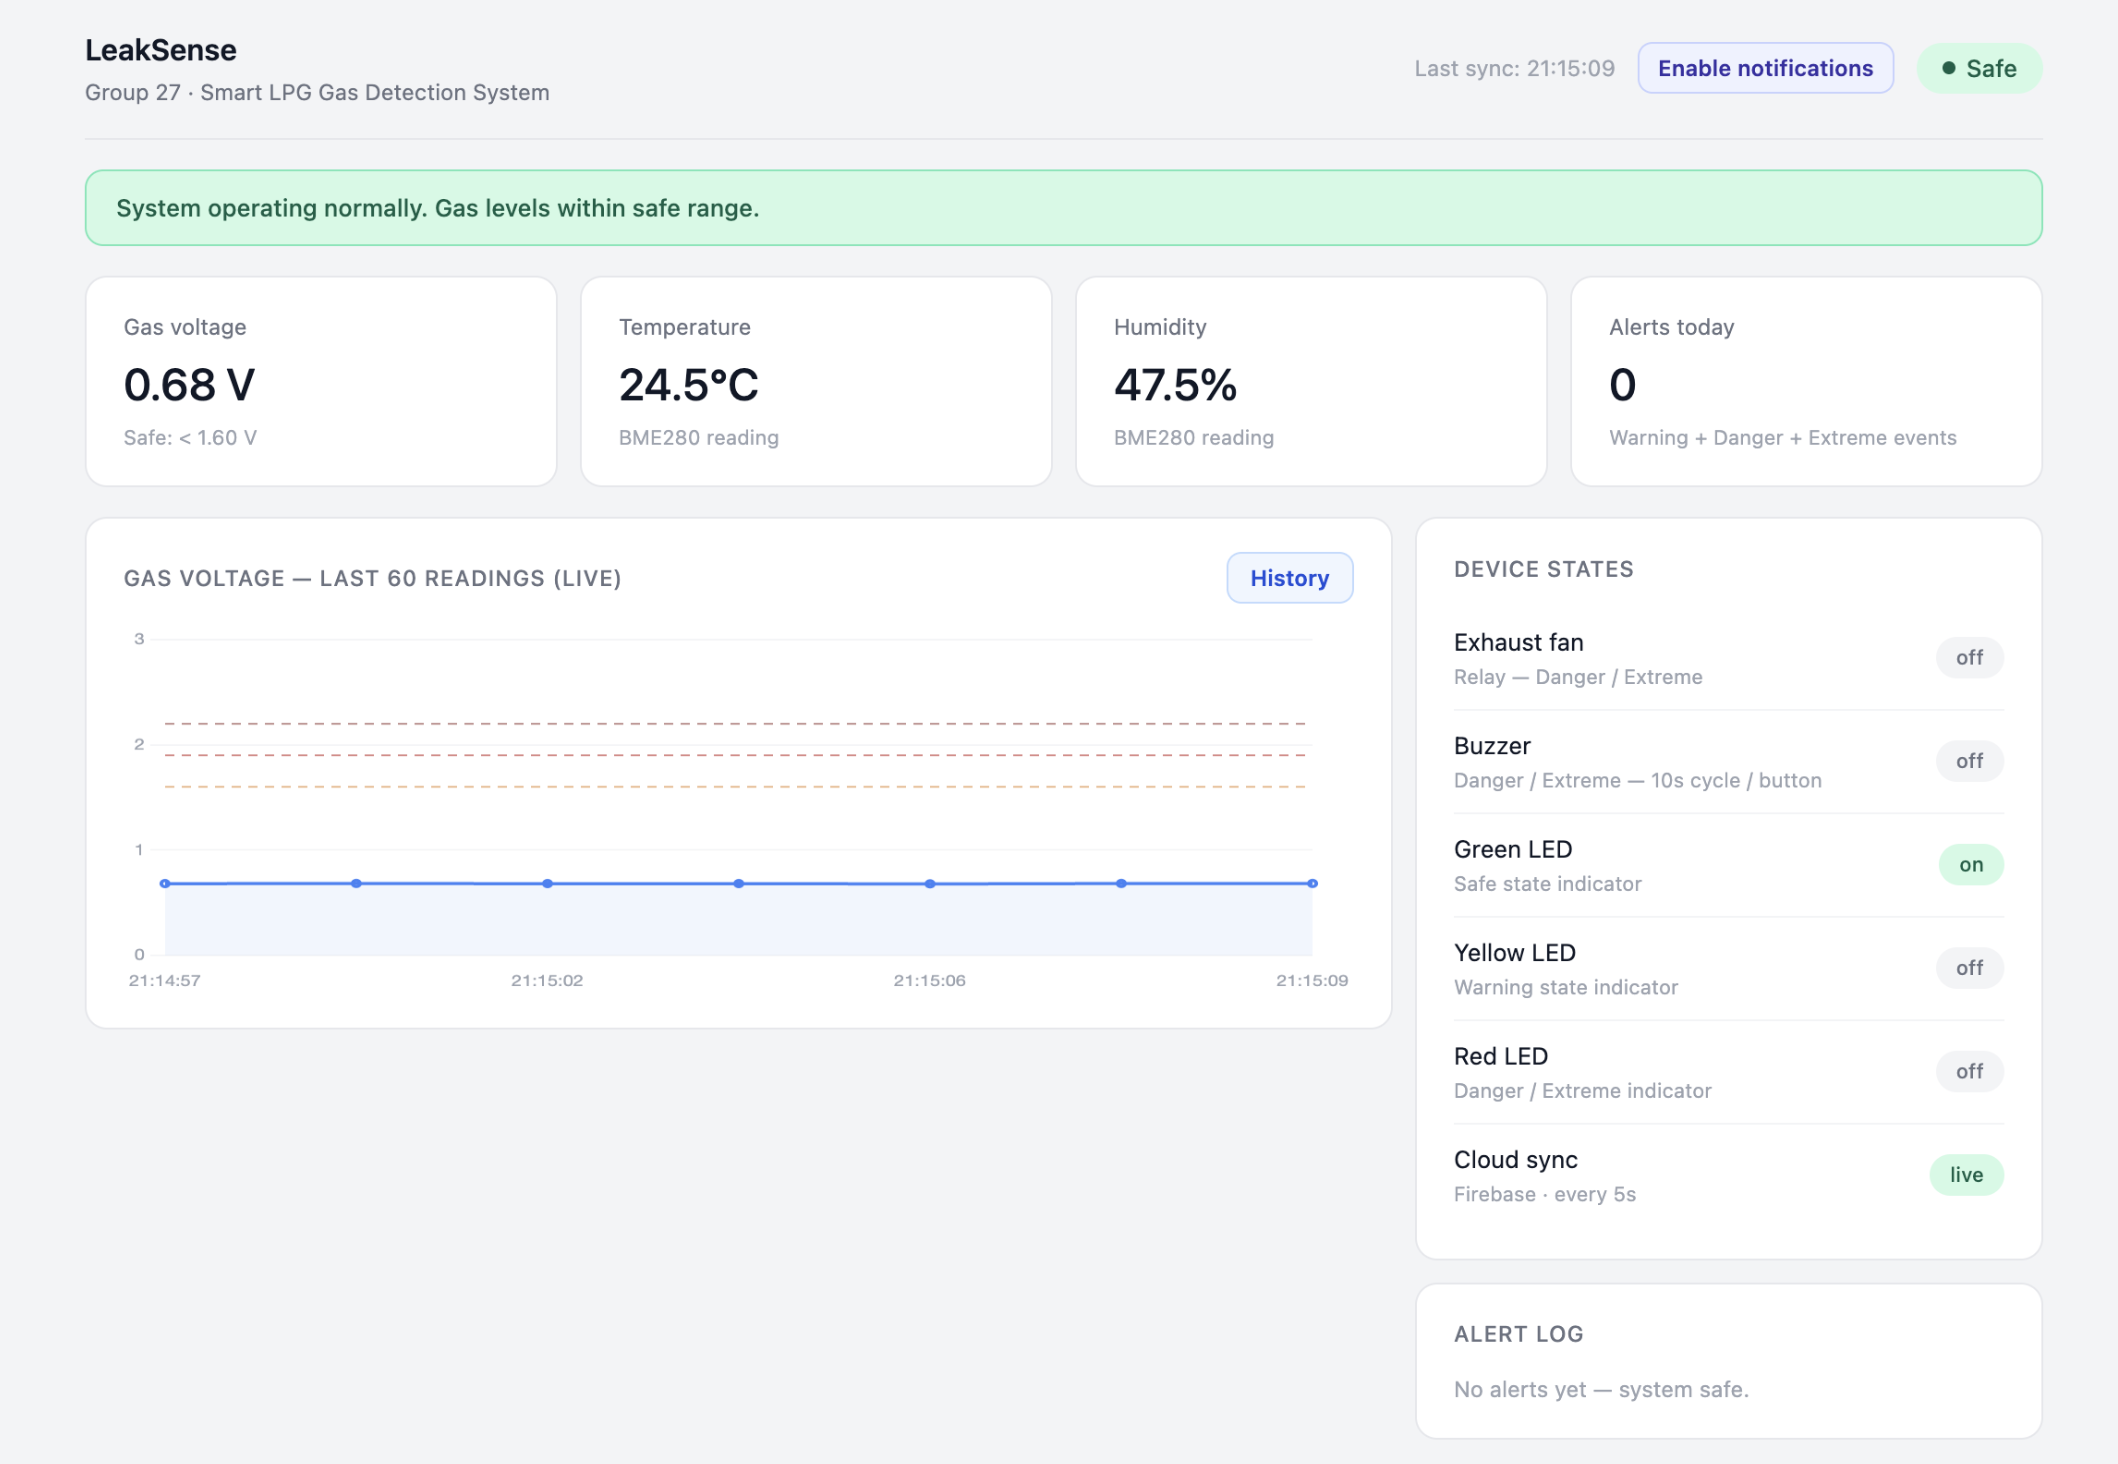
\includegraphics[width=0.7\linewidth]{normal_state.png}
  \caption{LeakSense web dashboard --- Safe state showing live gas voltage
  (0.68\,V), system status, device states panel, and live trend chart.}
  \label{fig:dash_safe}
\end{figure}

When the gas voltage rises into the 1.60--1.89\,V range, the dashboard changes
to Warning as shown in Fig.~\ref{fig:dash_warning}. At this level, the system
indicates elevated gas concentration but does not yet activate the fan or
buzzer. The warning view is useful because it gives the user an early visual
and remote indication before the system reaches the Danger threshold.

\begin{figure}[H]
  \centering
  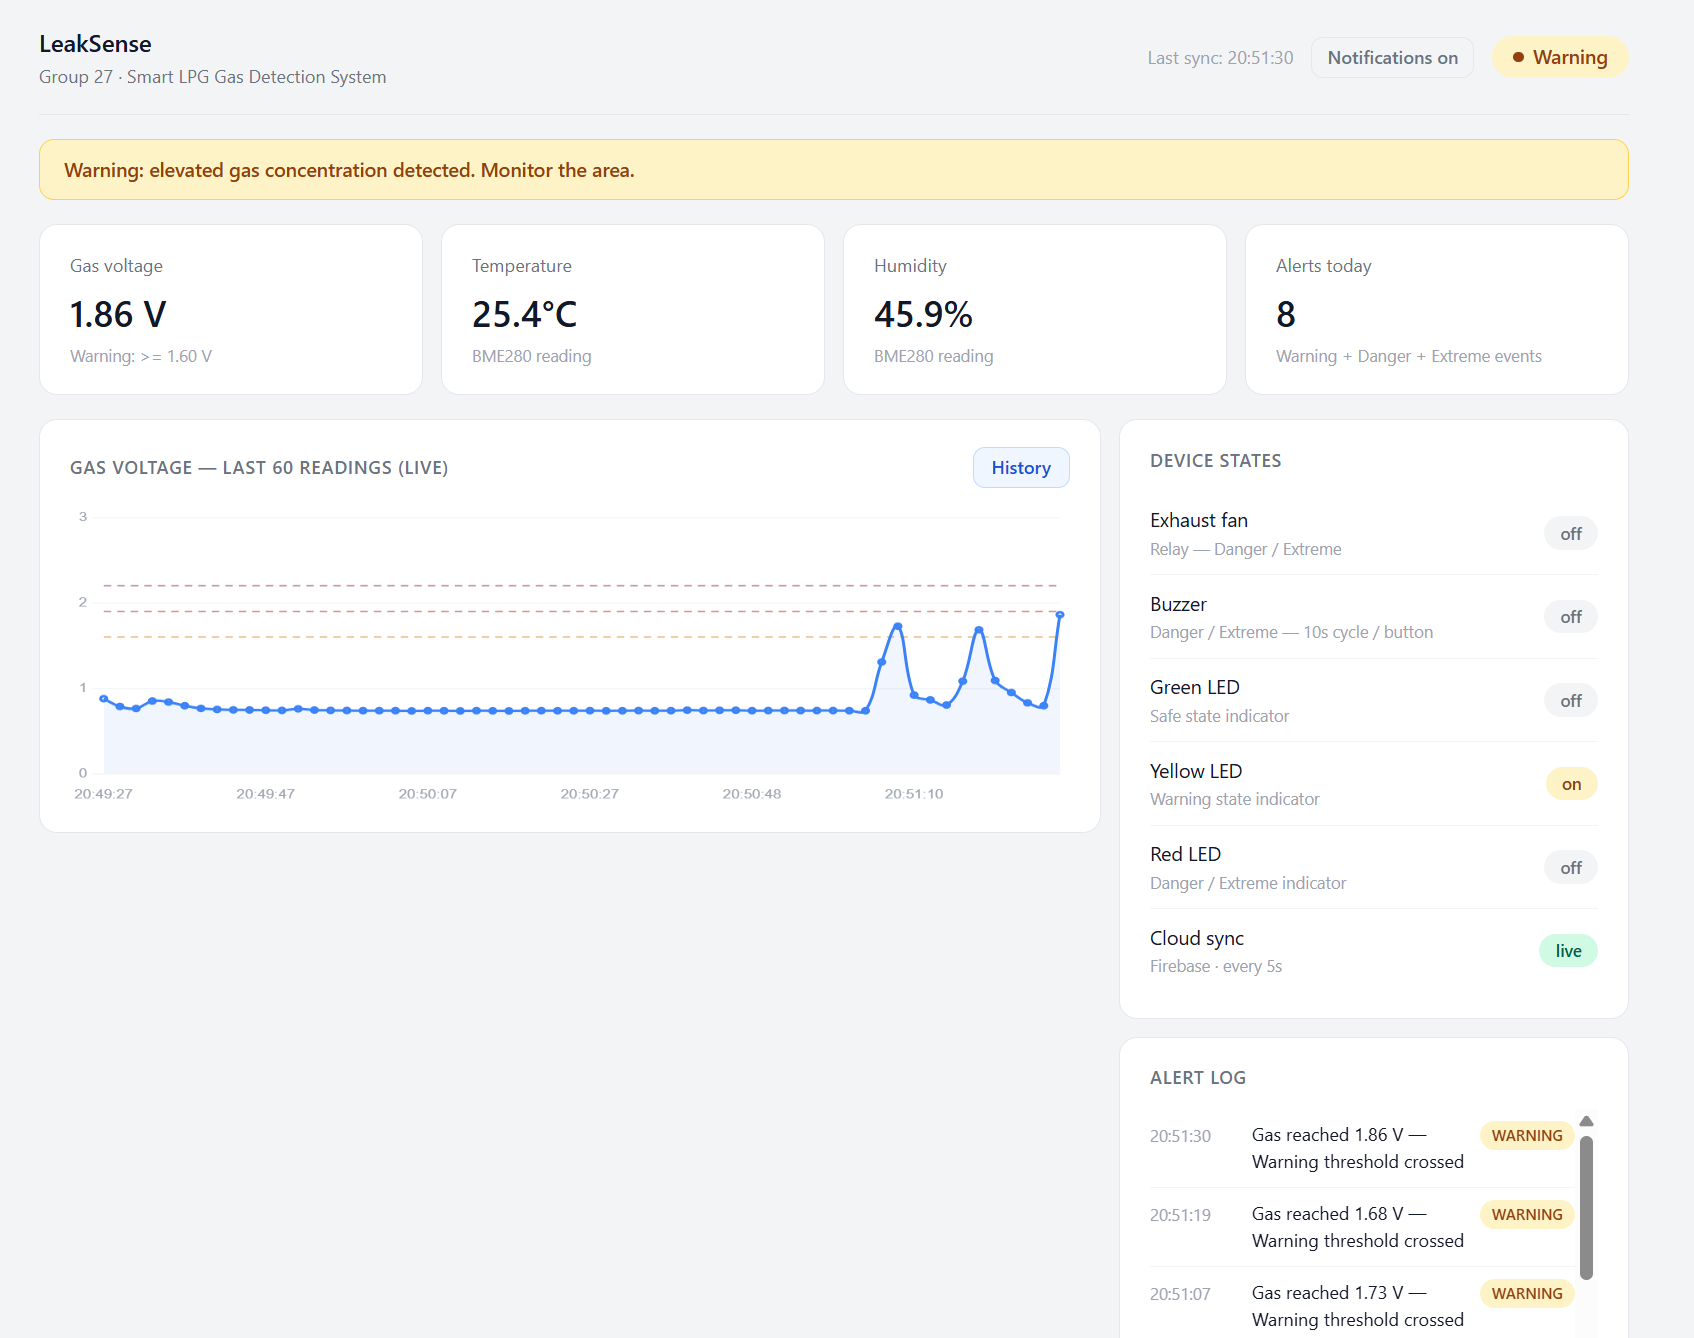
\includegraphics[width=0.7\linewidth]{warning_state.png}
  \caption{LeakSense web dashboard --- Warning state at 1.86\,V with
  Chrome push notification visible.}
  \label{fig:dash_warning}
\end{figure}

Fig.~\ref{fig:dash_danger} shows the Danger state, triggered when gas voltage
reaches 1.90\,V or above. In this state the dashboard confirms that the red LED
is active, the relay-driven fan is on, and the buzzer alarm cycle has started.
This matches the firmware behaviour and verifies that the cloud dashboard is
displaying the same safety state as the local hardware.

\begin{figure}[H]
  \centering
  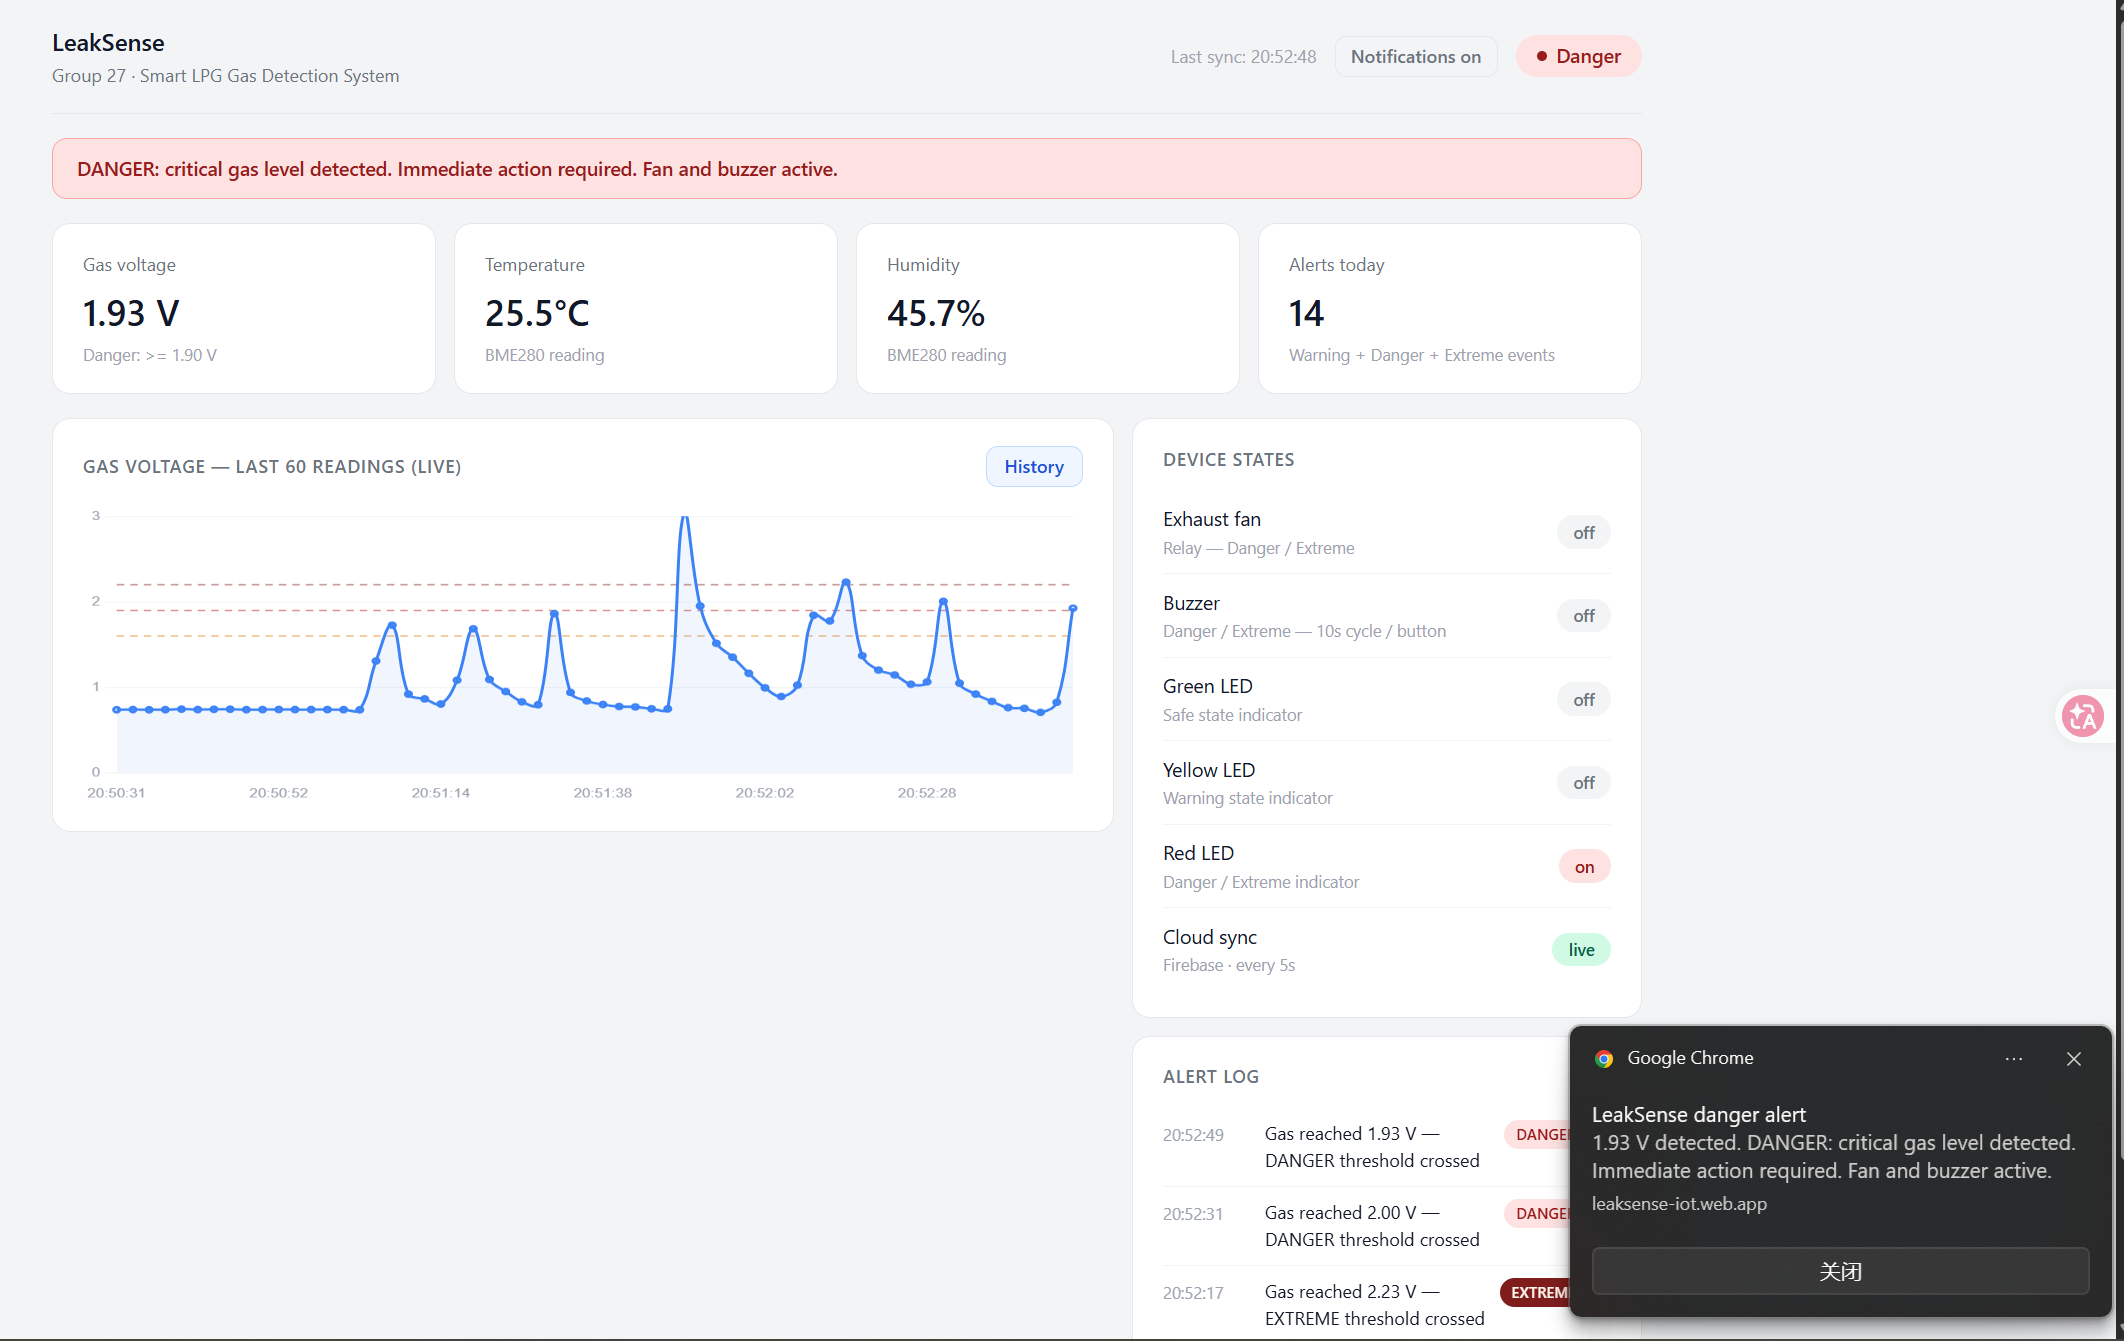
\includegraphics[width=0.7\linewidth]{danger_state.png}
  \caption{LeakSense web dashboard --- Danger state at 1.93\,V with
  Chrome push notification visible.}
  \label{fig:dash_danger}
\end{figure}


The Extreme view in Fig.~\ref{fig:dash_extreme} is a dashboard-level escalation
label for very high Danger readings above 2.20\,V. The firmware still treats
this condition as Danger, so the same local outputs remain active; however, the
dashboard uses the Extreme label to make the remote alert more urgent and
easier to distinguish from lower-level danger readings.

\begin{figure}[H]
  \centering
  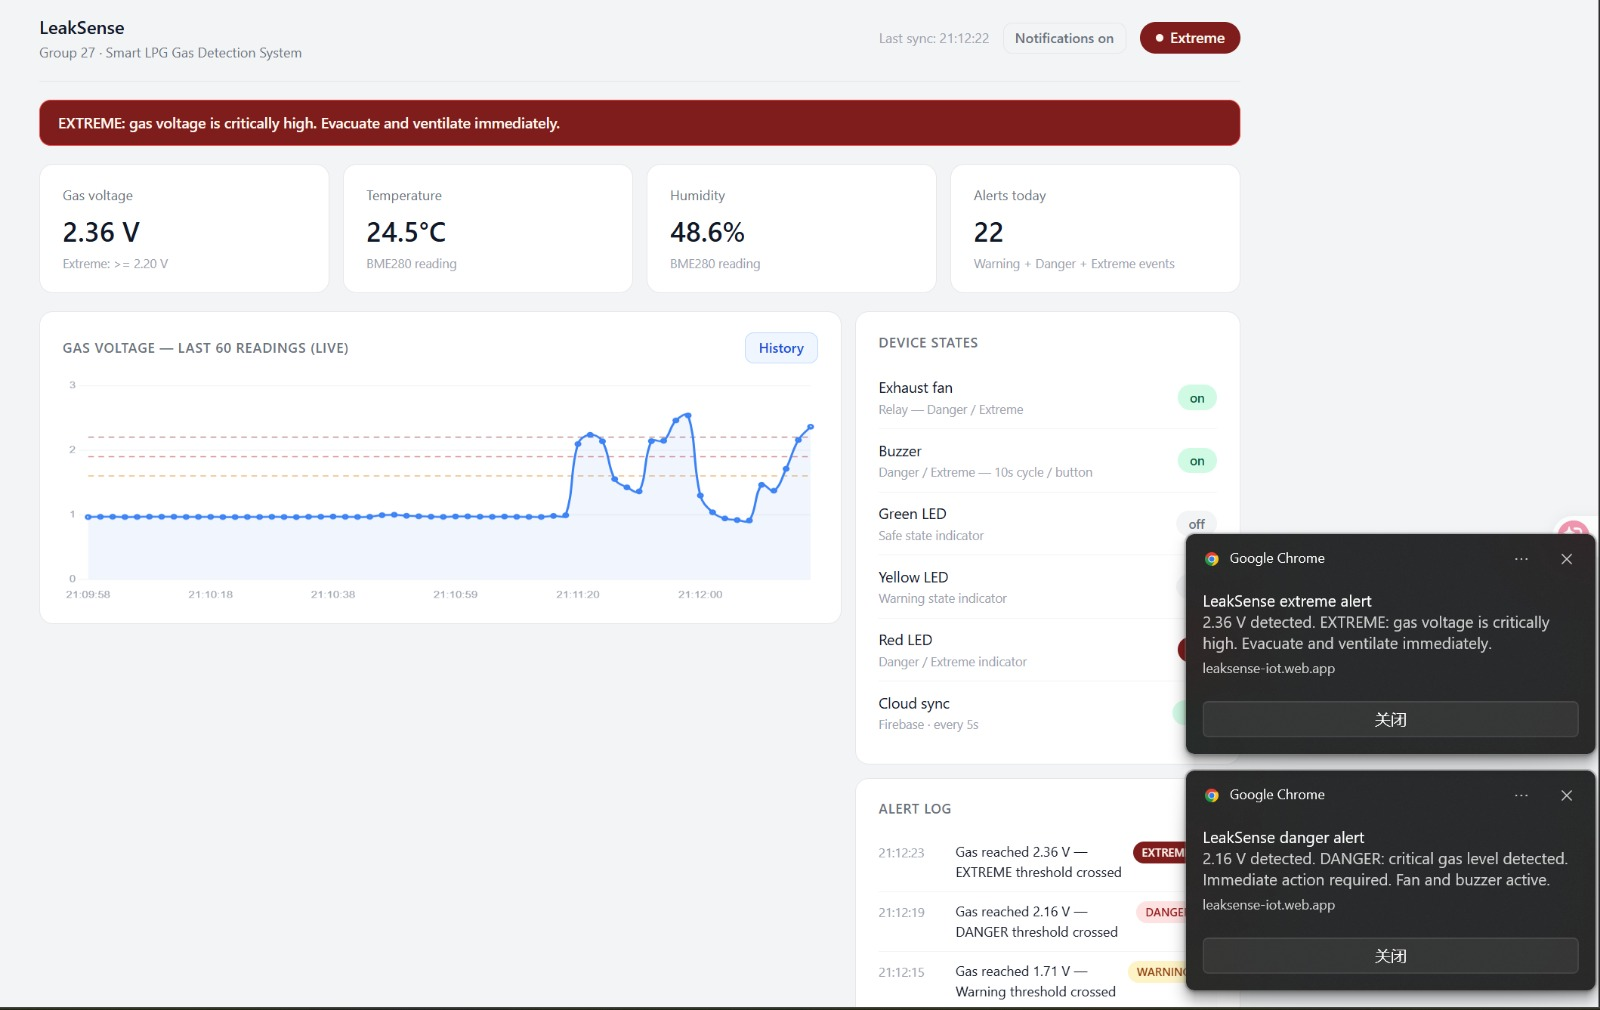
\includegraphics[width=0.7\linewidth]{extreme_state.jpeg}
  \caption{LeakSense web dashboard --- Extreme state at 2.36\,V with
  Chrome push notification visible.}
  \label{fig:dash_extreme}
\end{figure}

\subsection{24-Hour History View}

The history view complements the live dashboard by showing how gas voltage,
temperature, and humidity change over time. Rather than displaying only the
latest Firebase value, it reads records from \texttt{leaksense/history} and
plots the stored samples on a 24-hour chart. This helps identify recurring
patterns, such as repeated short warning events, sensor warm-up drift, or
environmental changes that coincide with gas readings.

\begin{figure}[H]
  \centering
  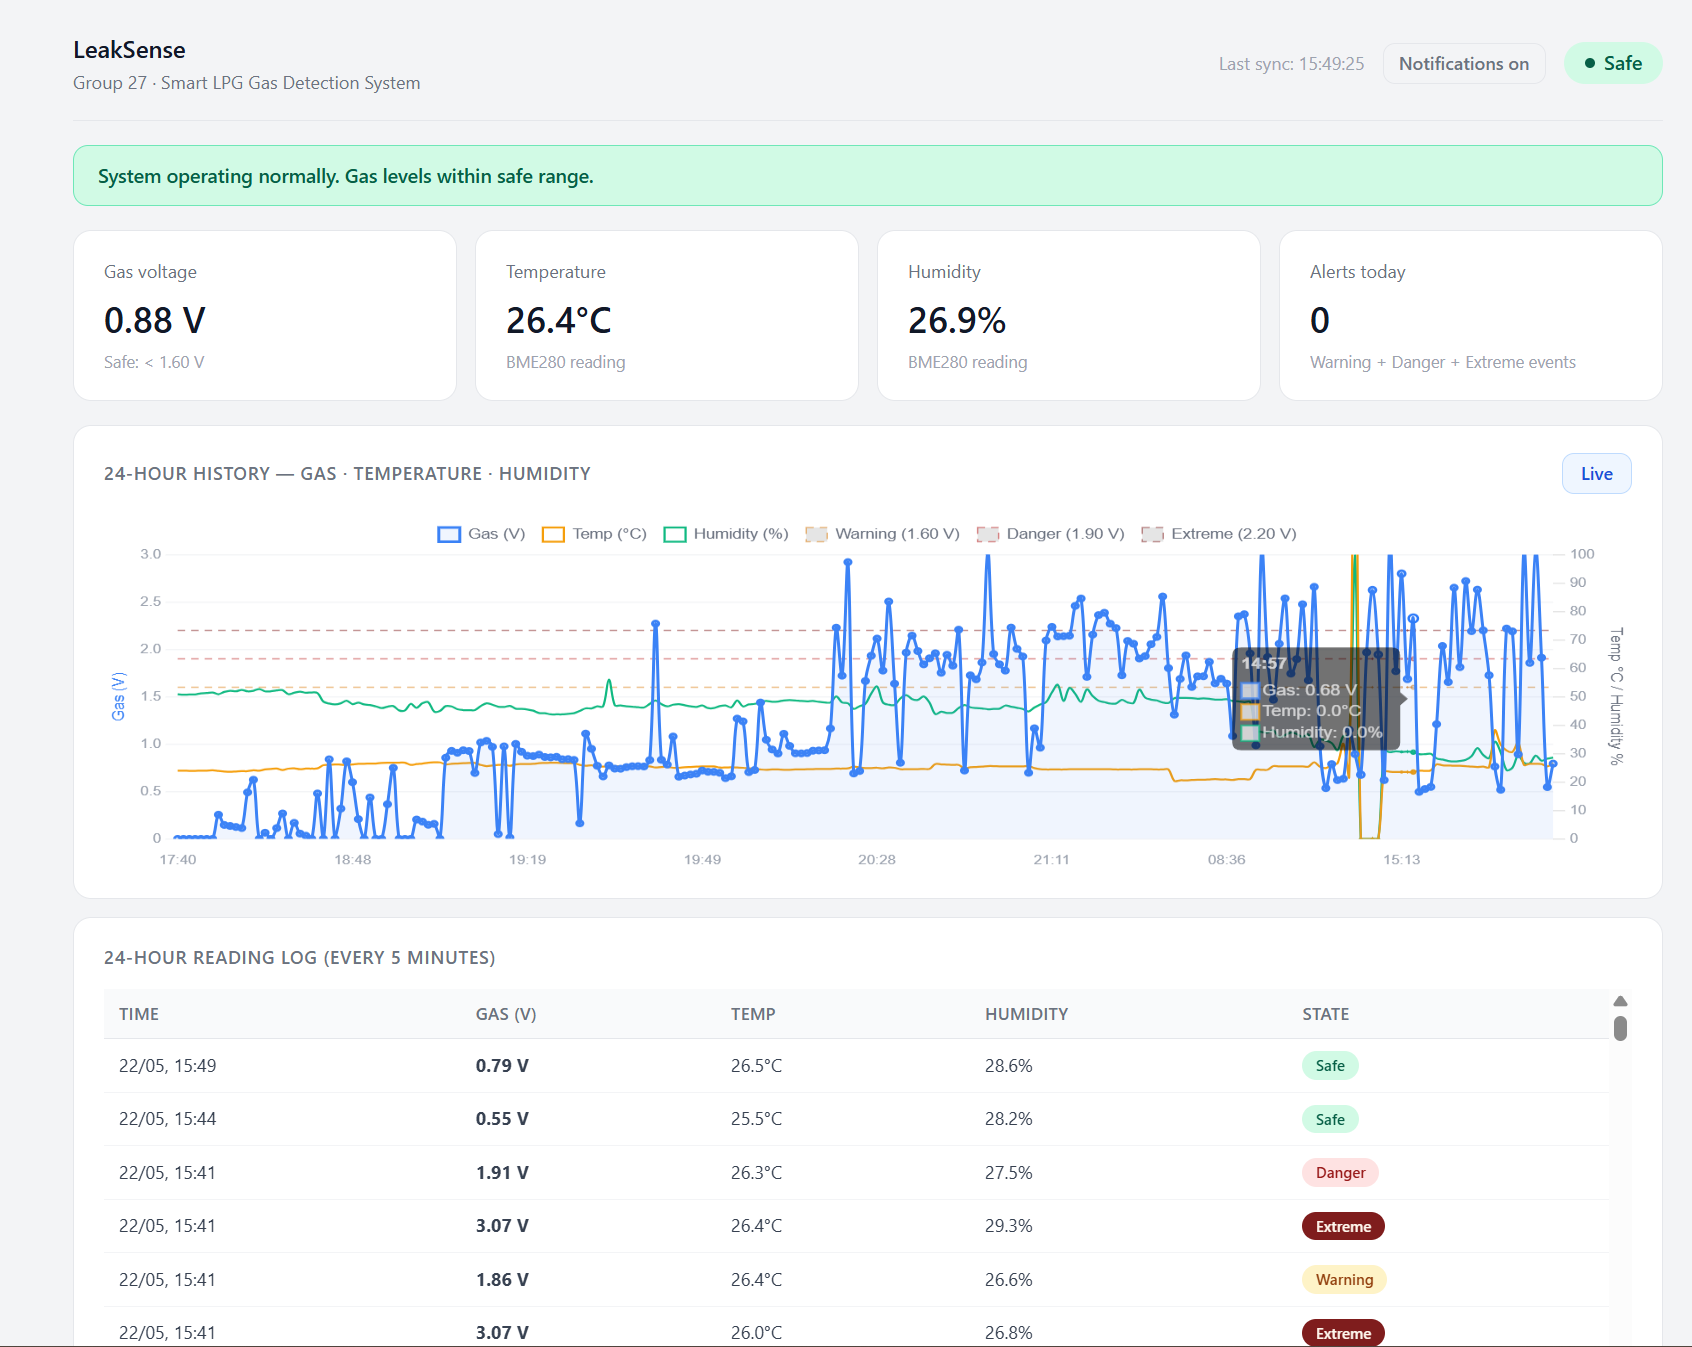
\includegraphics[width=0.7\linewidth]{24_hr_history.png}
  \caption{LeakSense 24-hour history view showing stored sensor readings and
  state changes over time.}
  \label{fig:history_24h}
\end{figure}

The table below the chart provides the same historical records in a readable
log format, including timestamp, voltage, environmental values, and state. This
is important for post-event analysis because a user can review when an alert
occurred, how long elevated readings persisted, and whether the temperature
trend supported the thermal escalation logic.


% ════════════════════════════════════════════════════════════════════════════
% VI. TESTING AND RESULTS
% ════════════════════════════════════════════════════════════════════════════
\section{Testing and Results}
\label{sec:testing}

\subsection{Testing Methodology}

Testing was conducted in four phases on the UWA IoT laboratory bench. The
SEN0565 sensor was allowed to warm up for a minimum of five minutes before
each test session, with the ten-second baseline period observed on every boot,
consistent with manufacturer warm-up guidance \cite{sen0565warmup}.

\textit{Phase~1} verified individual component communication: I2C addresses
were confirmed via serial monitor scan, sensor readings were checked against
expected ambient values, and actuator outputs were verified with a multimeter
and direct visual inspection.

\textit{Phase~2} tested state machine behaviour using butane lighter gas held
at measured distances from the sensor, recording the voltages at which state
transitions occurred. The thermal escalation logic was tested separately by
observing the temperature delta field across consecutive readings during
deliberate ambient temperature changes.

\textit{Phase~3} tested cloud communication by monitoring the Firebase console
during sensor operation and measuring the time between a reading being taken
and data appearing in the database.

\textit{Phase~4} tested the full end-to-end system including dashboard
responsiveness, push notification delivery, 24-hour history logging, and
behaviour during Wi-Fi disconnection.

\subsection{Test Results}

Table~\ref{tab:tests} summarises the results of the nine key test cases
conducted.

\begin{table}[H]
\centering
\caption{LeakSense test case results.}
\label{tab:tests}
\renewcommand{\arraystretch}{1.2}
\small
\setlength{\tabcolsep}{4pt}
\begin{tabularx}{\linewidth}{
  >{\centering\arraybackslash}p{0.7cm}
  >{\raggedright\arraybackslash}p{3.0cm}
  >{\raggedright\arraybackslash}X
  >{\raggedright\arraybackslash}X
  >{\centering\arraybackslash}p{1.2cm}
  >{\centering\arraybackslash}p{1.2cm}}
\toprule
\textbf{\#} & \textbf{Condition} & \textbf{Expected} & \textbf{Observed} &
\textbf{Time} & \textbf{Result} \\
\midrule
01 & Ambient air (baseline) & Safe $\cdot$ green LED on &
  Safe $\cdot$ 0.68\,V $\cdot$ green LED on & $<$1\,s & PASS \\
02 & Lighter gas --- moderate & Warning $\cdot$ yellow LED &
  Warning at 1.86\,V $\cdot$ yellow LED on & ${\sim}$2\,s & PASS \\
03 & Lighter gas --- sustained & Danger $\cdot$ fan + buzzer &
  Danger at 1.93\,V $\cdot$ fan + buzzer & ${\sim}$2\,s & PASS \\
04 & Lighter gas --- direct (stove) & Danger fw $\cdot$ Extreme display &
  2.36\,V $\cdot$ Extreme on dashboard & ${\sim}$2\,s & PASS \\
05 & Firebase latest push & Data within 2\,s &
  Confirmed in console $<$2\,s & $<$2\,s & PASS \\
06 & Dashboard live update & Update within 3\,s &
  Dashboard updated $<$3\,s & $<$3\,s & PASS \\
07 & Push notification & Chrome alert fires &
  Chrome notification received & ${\sim}$3\,s & PASS \\
08 & Wi-Fi disconnected mid-Danger & Local actuators continue &
  Fan + buzzer unaffected & 0\,s & PASS \\
09 & Button press during alarm & Silences current cycle &
  Buzzer off $\cdot$ restarts next cycle & $<$0.1\,s & PASS \\
\bottomrule
\end{tabularx}
\end{table}

\subsection{Results Analysis}

All nine test cases passed. The system correctly classified gas voltage into
all four display states and activated the appropriate actuators within the
two-second polling interval. The two-second response time is determined by
the sensor polling interval rather than processing latency --- classification
and actuator update execute in under one millisecond once the sensor reading
is available.

Firebase push latency of under two seconds is within the target and is
primarily determined by network round-trip time. Dashboard update latency of
under three seconds reflects the combined Firebase push latency and the
\texttt{onValue()} callback overhead. Push notification delivery at
approximately three seconds reflects additional service worker processing
time.

The Wi-Fi disconnection test confirmed the most important safety property of
the design: local actuators operate entirely independently of cloud
connectivity. When Wi-Fi was disabled during a Danger state, the fan and
buzzer continued operating and the OLED continued updating, while Firebase
push attempts were silently skipped. The button test confirmed that the
current buzzer cycle is silenced immediately on press but the subsequent
cycle restarts automatically when the gas remains in the Danger state.

The live demonstration using a gas stove (no ignition) confirmed real-world
operation: voltage climbed from a Safe baseline of 0.68\,V to 2.36\,V within
four seconds of the stove valve opening, triggering Danger and the Extreme
dashboard label, activating the fan and buzzer, and firing a Chrome push
notification before any team member present could detect the gas by smell.

% ════════════════════════════════════════════════════════════════════════════
% VII. LIMITATIONS AND FUTURE WORK
% ════════════════════════════════════════════════════════════════════════════
\section{Limitations and Future Work}
\label{sec:limitations}

\subsection{Current Limitations}

\subsubsection{Empirical Voltage Thresholds}
The most significant limitation is that the voltage thresholds (1.60\,V for
Warning, 1.90\,V for Danger) are empirical calibration constants determined
empirically during laboratory testing. The SEN0565 MEMS sensor is documented
by DFRobot as a qualitative sensor only --- it does not produce calibrated
concentration measurements \cite{sen0565wiki}. No manufacturer-published
voltage-to-concentration mapping exists for this sensor. For a production
safety system, formal calibration against certified LPG reference gas or a
known percentage-LEL standard (OSHA specifies propane LEL at 2.1\% by
volume \cite{osha2024}) would be required. The system architecture
accommodates recalibration: threshold constants are defined at the top of
the firmware source and can be updated without structural changes.

\subsubsection{Exhaust Fan Scale}
The exhaust fan used in LeakSense is a small 12\,V unit suitable for
demonstrating relay-controlled ventilation but would not provide sufficient
airflow to disperse LPG in a real room. A production system would require a
mains-powered exhaust fan or a direct connection to an existing kitchen
ventilation system.

\subsubsection{No Physical Gas Shutoff Valve}
The system activates ventilation and issues alerts but does not shut off the
gas supply at the source. A solenoid valve integrated into the LPG supply
line would provide a more complete safety response by eliminating the hazard
rather than only mitigating it.

\subsubsection{Firebase Security Configuration}
The database currently operates with open read/write rules appropriate for a
development configuration. A production deployment must implement Firebase
Authentication and restrict write access to the ESP32 device credential only,
with read access restricted to authenticated dashboard users.

\subsubsection{Single Sensor Node and No Battery Backup}
One gas sensor provides a single measurement point; a larger installation
would benefit from multiple nodes. The system has no battery backup --- a
mains power failure disables all monitoring and local safety responses.

\subsection{Future Work}

Planned improvements include: (1)~formal voltage-to-concentration calibration
using certified LPG test gas to establish defensible thresholds based on
percentage-LEL values; (2)~a solenoid shutoff valve on the LPG supply line
integrated with the existing relay driver circuit; (3)~a UPS module or
lithium battery backup for the ESP32; (4)~production-grade Firebase security
rules with device authentication; (5)~a multi-node sensor mesh using ESP-NOW
for larger residential spaces; (6)~Firebase Cloud Functions for automatic
history record pruning beyond 24 hours; and (7)~dashboard email and SMS alert
channels in addition to browser push notifications.


% ════════════════════════════════════════════════════════════════════════════
% VIII. PROJECT COST
% ════════════════════════════════════════════════════════════════════════════
\section{Project Cost}

Table~\ref{tab:cost} gives the component cost estimate. Components were sourced
from Core Electronics, Soldered, and Element14.

\begin{table}[H]
\centering
\caption{LeakSense component costs.}
\label{tab:cost}
\renewcommand{\arraystretch}{1.2}
\setlength{\tabcolsep}{2.5pt}
\scriptsize
\begin{tabularx}{\linewidth}{c
  >{\raggedright\arraybackslash}p{1.8cm}
  >{\raggedright\arraybackslash}X
  c
  >{\raggedleft\arraybackslash}p{0.8cm}
  >{\raggedright\arraybackslash}p{6.2cm}}
\toprule
\textbf{No.} & \textbf{Item} & \textbf{Description} & \textbf{Qty} &
\textbf{Cost} & \textbf{Web Address} \\
\midrule
1 & FireBeetle Board ESP32-E & Core controller with Wi-Fi and Bluetooth for
IoT communication. & 1 & \$18.80 &
\url{https://core-electronics.com.au/firebeetle-board-esp32-e-arduino-compatible.html} \\
2 & SEN0565 MEMS Methane CH4 Gas Detection Sensor & Primary gas sensing input
used for leakage detection. & 1 & \$8.55 &
\url{https://core-electronics.com.au/fermion-mems-methane-ch4-gas-detection-sensor-breakout-1-10000ppm.html} \\
3 & BME280 Atmospheric Sensor & Temperature, humidity, and pressure sensor used
to reduce false alarms. & 1 & \$23.50 &
\url{https://core-electronics.com.au/piicodev-atmospheric-sensor-bme280.html} \\
4 & OLED Display SSD1306 (I2C) & 0.96~in I2C SSD1306 screen for local status
and data monitoring. & 1 & \$7.20 &
\url{https://core-electronics.com.au/white-i2c-oled-display-ssd1306.html} \\
5 & 5\,V Relay Module & Switches the fan load from ESP32 GPIO and provides
electrical isolation. & 1 & \$3.95 &
\url{https://core-electronics.com.au/5v-single-channel-relay-module-10a.html} \\
6 & Delta 5\,V DC Exhaust Fan 40\,mm & 5\,V DC 40\,mm 3150~RPM fan used for
ventilation simulation. & 1 & \$16.50 &
\url{https://core-electronics.com.au/delta-electronics-frameless-fan-47192.html} \\
7 & Gravity Digital Buzzer Module & Gravity module used to provide audible
alerts and system warnings. & 1 & \$3.14 &
\url{https://core-electronics.com.au/digital-buzzer-module.html} \\
8 & 5\,mm LED & Visual state indicator. & 3 & \$3.14 &
\url{https://au.element14.com/broadcom-limited/hlmp-3507/led-5mm-green-4-2mcd-569nm/dp/1003214} \\
9 & Resistors (270~Ohm) & Current limiting for LEDs; 600-pack covers all
values. & 1 & \$2.95 &
\url{https://core-electronics.com.au/600-pack-of-1-4-watt-1-resistors-30-values-20-of-each.html} \\
10 & Breadboard 830 tie-pt & Prototyping platform for all connections. & 1 &
\$2.95 &
\url{https://core-electronics.com.au/solderless-breadboard-830-tie-point-zy-102.html} \\
11 & Jumper Wires M-M and M-F & Breadboard interconnects; M-F wires are used
for sensor modules and the OLED. & 1 & \$3.59 &
\url{https://core-electronics.com.au/solderless-breadboard-jumper-cable-wires-75-pieces.html} \\
\midrule
\multicolumn{4}{r}{\textbf{Total}} & \textbf{\$94.27} & \\
\bottomrule
\end{tabularx}
\end{table}

Competing commercial products provide context for this cost. The Aqara Smart
Gas Detector (AUD~\$130) detects methane, not LPG. The Google Nest Protect
(AUD~\$189) detects smoke and carbon monoxide, not LPG. The Honeywell BW
Solo detects LPG but has no auto ventilation and costs approximately
AUD~\$700. The Flowtech safety system includes a shutoff valve but starts at
AUD~\$1,500 and is designed for commercial installations. LeakSense delivers
LPG detection, relay-driven fan ventilation, cloud monitoring, 24-hour
history, and browser push notifications for approximately AUD~\$94. The thermal escalation
logic --- gas plus temperature risk combined --- is absent from every
commercial alternative listed above.

% ════════════════════════════════════════════════════════════════════════════
% IX. CONCLUSION
% ════════════════════════════════════════════════════════════════════════════
\section{Conclusion}
\label{sec:conclusion}

LeakSense demonstrates that an affordable, integrated residential LPG safety system 
can be built from commodity IoT components for approximately AUD~\$94 — roughly one-seventh 
the cost of the nearest commercial product with comparable functionality, and one-sixteenth the cost 
of systems offering certified shutoff integration. LeakSense integrates a MEMS analog gas sensor, 
a BME280 atmospheric sensor, relay-driven actuators, an ESP32 microcontroller, Firebase Realtime Database 
over HTTPS REST, and a browser-accessible dashboard with 24-hour history and push notifications into a coherent five-layer IoT architecture.

The four design goals defined in Section II were achieved and verified through 
nine test cases. Voltage-based state classification correctly identified Safe, 
Warning, Danger, and Extreme conditions at every tested threshold. The thermal escalation 
logic correctly promoted Warning to Danger when a temperature rise of 5 °C or higher 
coincided with elevated gas readings, supporting the dual-sensor approach as a practical 
mechanism for distinguishing pure gas events from combined gas-and-heat events. 
Actuators responded within the two-second polling interval, cloud-to-dashboard 
latency remained under three seconds, and the Wi-Fi disconnection test confirmed 
the project's most important safety property: all local actuation continues 
independently of cloud connectivity.

Beyond the working system, the project contributes a reproducible reference architecture 
for low-cost residential safety IoT. The separation of time-critical safety logic on the 
microcontroller from non-critical telemetry and visualisation in the cloud is a pattern 
that generalises to other household hazard domains, including smoke, carbon monoxide, 
and water leak detection. The empirical voltage thresholds, small-scale fan, and absence 
of a physical shutoff valve are acknowledged limitations rather than design flaws; each has 
a defined remediation path in Section VII, and none require structural redesign of the existing architecture.


For practitioners, the principal takeaway is that the technical gap between affordable 
consumer detectors and certified industrial systems is smaller than current market pricing 
implies. With formal calibration against a certified LPG reference, a mains-rated exhaust fan, 
a solenoid shutoff valve, and production-grade Firebase security rules, the LeakSense architecture 
provides a credible foundation for a deployable open residential gas safety product.

% ════════════════════════════════════════════════════════════════════════════
% X. HOW-TO GUIDE
% ════════════════════════════════════════════════════════════════════════════
\section{How-To Guide}
\label{sec:howto}

This guide describes how to assemble, configure, and run LeakSense from
scratch.

\subsection{Hardware Setup}

\begin{enumerate}
  \item Connect the SEN0565 gas sensor analog output to GPIO~39. Connect VCC
        to 3.3\,V and GND to GND.
  \item Connect the OLED SSD1306 to I2C Bus~0: SDA to GPIO~18, SCL to
        GPIO~23. Connect VCC to 3.3\,V.
  \item Connect the BME280 to I2C Bus~1: SDA to GPIO~22, SCL to GPIO~21.
        Connect VCC to 3.3\,V.
  \item Connect the HL-52S relay IN1 signal pin to GPIO~26. Connect the relay
        NO terminal in series with the fan's positive supply.
  \item Connect the buzzer signal pin to GPIO~25.
  \item Connect the green LED anode through a 270\,$\Omega$ resistor to
        GPIO~17, cathode to GND.
  \item Connect the yellow LED anode through a 270\,$\Omega$ resistor to
        GPIO~16, cathode to GND.
  \item Connect the red LED anode through a 270\,$\Omega$ resistor to GPIO~4,
        cathode to GND.
  \item Connect one terminal of the push button to GPIO~14, the other to GND.
        The firmware enables the internal pull-up resistor.
  \item Power the ESP32 via USB-C. Verify I2C connections using the serial
        monitor I2C scan output before uploading firmware.
\end{enumerate}

\subsection{Firmware Installation}

\begin{enumerate}
  \setcounter{enumi}{10}
  \item Install VS~Code and the PlatformIO IDE extension.
  \item Open the \texttt{firmware/} folder as a PlatformIO project.
  \item Copy \texttt{firmware/blinking/src/secrets.h.example} to
        \texttt{firmware/blinking/src/secrets.h} and fill in:
        \texttt{WIFI\_SSID}, \texttt{WIFI\_PASSWORD},
        \texttt{FIREBASE\_HOST}, and \texttt{FIREBASE\_AUTH}.
  \item Ensure the following are listed in \texttt{platformio.ini} under
        \texttt{lib\_deps}: Adafruit GFX Library, Adafruit SSD1306, Adafruit
        BME280 Library, and \texttt{mobizt/Firebase~ESP32~Client}.
  \item Click the PlatformIO Upload button to compile and flash the firmware.
  \item Open the Serial Monitor at 115200~baud. Allow five minutes for sensor
        warm-up before trusting readings.
\end{enumerate}

\subsection{Firebase Setup}

\begin{enumerate}
  \setcounter{enumi}{16}
  \item Go to \url{firebase.google.com} and create a project named
        \texttt{leaksense-iot}.
  \item Enable Realtime Database in test mode.
  \item In Project Settings $\to$ Service Accounts $\to$ Database Secrets,
        copy the database secret into the local firmware
        \texttt{secrets.h} file as \texttt{FIREBASE\_AUTH}.
  \item Copy the \texttt{databaseURL} from Project Settings and paste it
        (without \texttt{https://}) into the same \texttt{secrets.h} file as
        \texttt{FIREBASE\_HOST}.
  \item Set database rules to allow read and write for development. Update
        rules before any production deployment.
\end{enumerate}

\subsection{Dashboard Setup}

\begin{enumerate}
  \setcounter{enumi}{21}
  \item Copy \texttt{dashboard/js/secrets.example.js} to
        \texttt{dashboard/js/secrets.js}. The local \texttt{secrets.js} file is
        ignored by Git and should not be committed.
  \item Paste the Firebase web config object from Project Settings $\to$
        General $\to$ Your apps into \texttt{dashboard/js/secrets.js}.
  \item Open \texttt{dashboard/index.html} in a browser. The dashboard
        connects to Firebase automatically and displays live data.
  \item To enable push notifications, open the dashboard in Chrome and click
        Enable Notifications. Accept the browser permission prompt.
        Notifications will fire for Warning, Danger, and Extreme events.
  \item The 24-hour history view is accessible by clicking the History button
        on the live chart.
\end{enumerate}

% ════════════════════════════════════════════════════════════════════════════
% REFERENCES
% ════════════════════════════════════════════════════════════════════════════
\section*{References}
\label{sec:references}

\begingroup
\renewcommand{\refname}{}
\begin{thebibliography}{00}

\bibitem{gasEnergy2020}
Frontier Economics, ``Gas Vision 2050: Delivering a Clean Energy Future,'' 
Gas Energy Australia, Sep. 2020. [Online]. Available: 
\url{https://www.gasenergyaus.au/get/1868/gas-vision-2050-frontier-economics-september.pdf}. 
[Accessed: May 2026].


\bibitem{fireRescue2023}
Fire and Rescue NSW, ``Annual Report 2024--25,'' Fire and Rescue NSW, Oct. 2025. 
[Online]. Available: 
\url{https://www.fire.nsw.gov.au/\_\_data/assets/pdf\_file/0022/4936/annual\_report\_2024\_25.pdf}. 
[Accessed: May 2026].


\bibitem{islam2020}
M.~R. Islam \textit{et al.}, ``IoT-based smart gas leakage detection and
safety system using wireless sensor networks,'' \textit{IEEE Access}, vol.~8,
pp.~201360--201371, 2020, doi:~10.1109/ACCESS.2020.3035486.

\bibitem{sarkar2024}
R.~Sarkar \textit{et al.}, ``Elevating Gas Safety Standards: ESP32-based
Detection Systems with Blynk Integration,'' in \textit{Proc. 2024 IEEE Region
10 Symposium (TENSYMP)}, 2024.

\bibitem{sen0565wiki}
DFRobot, ``SEN0565 Fermion MEMS CH4 Gas Detection Sensor Wiki,'' DFRobot,
2024. [Online]. Available: \url{https://wiki.dfrobot.com/sen0565}.
[Accessed: May 2026].

\bibitem{sen0565warmup}
DFRobot, ``SEN0565 Raw Reading Example --- warm-up guidance,'' DFRobot, 2024.
[Online]. Available: \url{https://wiki.dfrobot.com/sen0565/docs/18020}.
[Accessed: May 2026].

\bibitem{osha2024}
OSHA, ``LPG Chemical Data --- Lower Explosive Limit,'' United States Department
of Labor, 2024. [Online]. Available:
\url{https://www.osha.gov/chemicaldata/484}. [Accessed: May 2026].

\bibitem{wu2021}
L.~Wu, L.~Chen, and X.~Hao, ``Multi-sensor data fusion algorithm for early
indoor fire warning based on BP neural network,'' \textit{Information},
vol.~12, no.~2, p.~59, 2021.

\bibitem{espressif2026}
Espressif Systems, ``ESP32 Technical Reference Manual,'' Espressif Systems,
2026. [Online]. Available:
\url{https://www.espressif.com/sites/default/files/documentation/esp32_technical_reference_manual_en.pdf}.
[Accessed: May 2026].

\bibitem{bme280}
Bosch Sensortec, ``BME280 Combined Humidity and Pressure Sensor --- Data Sheet,'' 
Document BST-BME280-DS002, Rev. 1.6, Sep. 2018. [Online]. Available: 
\url{https://www.bosch-sensortec.com/media/boschsensortec/downloads/datasheets/bst-bme280-ds002.pdf}. 
[Accessed: May 2026].

\bibitem{firebase2024}
Google Firebase, ``Firebase Realtime Database Documentation,'' Google, 2024.
[Online]. Available: \url{https://firebase.google.com/docs/database}.
[Accessed: May 2026].

\bibitem{saeed2018}
F. Saeed, A. Paul, A. Rehman, W. H. Hong, and H. Seo, ``IoT-based intelligent 
modeling of smart home environment for fire prevention and safety,'' 
\emph{J. Sensor Actuator Networks}, vol. 7, no. 1, p. 11, Mar. 2018, 
doi: 10.3390/jsan7010011. [Online]. Available: \url{https://www.mdpi.com/2224-2708/7/1/11}. 
[Accessed: May 2026].

\bibitem{ssd1306core}
Core Electronics, ``White I2C OLED Display (SSD1306),'' Core Electronics, 
2020. [Online]. Available: 
\url{https://core-electronics.com.au/white-i2c-oled-display-ssd1306.html}. 
[Accessed: May 2026].

\bibitem{gravitybuzzer}
DFRobot, ``Gravity: Digital Buzzer Module,'' DFRobot Wiki, 2024. [Online]. 
Available: \url{https://wiki.dfrobot.com/dfr0032/}. [Accessed: May 2026].

\bibitem{hl52srelay}
Core Electronics, ``5V Single Channel Relay Module 10A,'' Core Electronics, 
2024. [Online]. Available: 
\url{https://core-electronics.com.au/5v-single-channel-relay-module-10a.html}. 
[Accessed: May 2026].

\bibitem{deltafan}
Core Electronics, ``Delta Electronics Frameless Fan,'' Core Electronics, 
2024. [Online]. Available: 
\url{https://core-electronics.com.au/delta-electronics-frameless-fan-47192.html}. 
[Accessed: May 2026].

\bibitem{breadboard830}
Core Electronics, ``Solderless Breadboard 830 Tie-Point ZY-102,'' Core 
Electronics, 2024. [Online]. Available: 
\url{https://core-electronics.com.au/solderless-breadboard-830-tie-point-zy-102.html}. 
[Accessed: May 2026].

\end{thebibliography}
\endgroup

% ════════════════════════════════════════════════════════════════════════════
% APPENDICES
% ════════════════════════════════════════════════════════════════════════════
\appendices

\section{Code Function Explanations}
\label{sec:coding}

The code function explanations and source listings document the implementation
used by LeakSense. The same source code is also available in the
project GitHub repository:
\url{https://github.com/sahilppatel1807/CITS5506-LeakSense-IoT}. For hardware
assembly, firmware upload, Firebase setup, and dashboard operation instructions,
see the How-To Guide.

\subsection{Code Organisation}

The LeakSense implementation is divided into embedded firmware and browser
dashboard code. The embedded firmware is stored in
\path{firmware/blinking/} and runs on the FireBeetle ESP32-E using
PlatformIO and the Arduino framework. The dashboard is stored in
\path{dashboard/} and runs as a plain HTML, CSS, and JavaScript application
connected to Firebase Realtime Database. This split keeps time-critical safety
logic on the ESP32 and presentation logic in the browser.

Table~\ref{tab:codefiles} summarises the files included in Appendix~B. The
source listings are included directly from the repository so the report shows
the same code used by LeakSense.

\begin{table}[H]
\centering
\caption{LeakSense source files included in Appendix~B.}
\label{tab:codefiles}
\renewcommand{\arraystretch}{1.2}
\setlength{\tabcolsep}{6pt}
\begin{tabularx}{\linewidth}{
  >{\raggedright\arraybackslash}p{5.0cm}
  >{\raggedright\arraybackslash}X}
\toprule
\textbf{File} & \textbf{Role} \\
\midrule
\path{firmware/blinking/src/main.cpp} & ESP32 firmware: sensors, state machine,
actuators, OLED display, Wi-Fi, Firebase REST upload. \\
\path{firmware/blinking/platformio.ini} & PlatformIO board, framework, monitor,
and library dependency configuration. \\
\path{firmware/blinking/src/secrets.h.example} & Template for private Wi-Fi and
Firebase credentials. \\
\path{dashboard/index.html} & Dashboard page structure and UI elements. \\
\path{dashboard/css/style.css} & Dashboard layout, state colours, cards,
buttons, tables, and responsive styling. \\
\path{dashboard/js/secrets.example.js} & Template for the local Firebase web
configuration file used by the dashboard. \\
\path{dashboard/js/firebase.js} & Firebase setup, database listeners, and data
normalisation. \\
\path{dashboard/js/dashboard.js} & Main dashboard state handling, alert log,
notifications, and DOM updates. \\
\path{dashboard/js/charts.js} & Chart.js live trend and 24-hour history charts. \\
\path{dashboard/js/mock.js} & Simulated readings for testing the dashboard
without live hardware. \\
\path{dashboard/service-worker.js} & Browser notification service worker. \\
\bottomrule
\end{tabularx}
\end{table}

\subsection{Firmware Functions Explained}

The firmware is written with descriptive constants and small functions so that
each hardware responsibility is visible in the code. Pin numbers, timing
intervals, thresholds, active-low polarity, and calibration values are declared
at the top of \texttt{main.cpp}. This makes the safety thresholds and GPIO
assignments easy to audit and change.

The most important firmware functions are:
\begin{itemize}
  \item \texttt{setup()} initialises GPIO, runs the LED self-test, configures
        ADC resolution, scans both I2C buses, initialises the OLED and BME280,
        and starts Wi-Fi connection in the background.
  \item \texttt{loop()} is the main cooperative scheduler. It services alarm
        controls and Wi-Fi continuously, then performs a complete sensor,
        classification, actuator, Firebase, and OLED update every two seconds.
  \item \texttt{readAnalogVoltage()} averages 32 ADC samples from the SEN0565
        gas sensor, reducing noise before state classification.
  \item \texttt{updateGasBaseline()} tracks the clean-air baseline slowly when
        readings remain stable, but avoids learning elevated gas readings as
        normal.
  \item \texttt{evaluateGasLevel()} converts gas voltage into Safe, Warning, or
        Danger using the fixed thresholds.
  \item \texttt{confirmGasLevel()} prevents noisy single-sample danger spikes
        from triggering ordinary Danger, while allowing immediate Danger when
        the reading exceeds the Extreme voltage threshold.
  \item \texttt{hasThermalRisk()} checks whether the BME280 temperature has
        risen by at least 5\,$^{\circ}$C between readings or reached
        55\,$^{\circ}$C absolute.
  \item \texttt{startDangerAlarm()}, \texttt{updateDangerAlarm()}, and
        \texttt{stopDangerAlarm()} control the buzzer and fan alarm cycle.
  \item \texttt{handleAlarmCancelButton()} handles the GPIO~14 push button and
        pauses detection temporarily after user acknowledgement.
  \item \texttt{firebasePayload()}, \texttt{uploadLatestToFirebase()}, and
        \texttt{uploadHistoryToFirebase()} build JSON records and send them to
        Firebase using HTTPS REST calls.
  \item \texttt{drawStatusScreen()} renders local OLED status including
        temperature, humidity, gas voltage, baseline, state, alarm, and fan
        status.
\end{itemize}

The firmware comments explain why timing, baselining, and upload behaviour are
implemented in this way. The most important safety choice is that actuator
updates occur before Firebase communication, so the fan, buzzer, and LEDs do
not depend on Wi-Fi or cloud availability.

\subsection{Dashboard Functions Explained}

The dashboard JavaScript separates Firebase input, UI state handling, charts,
and mock data. This makes it possible to test the browser interface without
the ESP32 while keeping the same internal reading format.

The key dashboard functions are:
\begin{itemize}
  \item \texttt{secrets.example.js} shows the required Firebase web
        configuration fields. The real local file is named
        \texttt{secrets.js} and is ignored by Git so project details are not
        committed.
  \item \texttt{normaliseReading()} in \texttt{firebase.js} converts Firebase
        records into one consistent object shape, handling missing fields,
        legacy names, booleans, numbers, timestamps, and state classification.
  \item \texttt{listenToSensorData()} subscribes to
        \texttt{leaksense/latest} so the dashboard updates in real time when
        the ESP32 uploads a new reading.
  \item \texttt{loadHistory()} and \texttt{listenToHistory()} read and stream
        \texttt{leaksense/history} records for the 24-hour history view.
  \item \texttt{onNewReading()} in \texttt{dashboard.js} is the main UI update
        function. It updates the state badge, banner, metrics, device state
        pills, live chart, alert log, and notifications.
  \item \texttt{sendAlertNotification()} creates browser notifications for
        Warning, Danger, and Extreme events.
  \item \texttt{setupDashboardViews()} switches between the live dashboard and
        24-hour history views.
  \item \texttt{initChart()}, \texttt{updateChart()},
        \texttt{initHistoryChart()}, and \texttt{addHistoryPoint()} in
        \texttt{charts.js} create and update the Chart.js visualisations.
  \item \texttt{getMockReading()} in \texttt{mock.js} produces simulated gas,
        temperature, humidity, actuator, and state values when hardware data is
        unavailable.
\end{itemize}

The HTML file defines the visible dashboard structure, the CSS file defines
the state-specific visual design, and the JavaScript files apply the live
Firebase data to those elements.

\section{Source Code Listings}
\label{sec:source-code-listings}

\begingroup
\setlength{\columnsep}{24pt}
\setlength{\columnseprule}{0.3pt}
\lstset{style=leaksensecodecompact}
\begin{multicols}{2}

\subsection{Firmware Source Code}

\leaksensecompactlisting[language=C++]{ESP32 firmware source code: firmware/blinking/src/main.cpp.}{lst:firmware-main}{../firmware/blinking/src/main.cpp}

\subsection{PlatformIO Configuration}

\leaksensecompactlisting{PlatformIO configuration: firmware/blinking/platformio.ini.}{lst:platformio}{../firmware/blinking/platformio.ini}

\subsection{Credential Template}

\leaksensecompactlisting[language=C++]{Credential template: firmware/blinking/src/secrets.h.example.}{lst:secrets-example}{../firmware/blinking/src/secrets.h.example}

\subsection{Dashboard HTML}

\leaksensecompactlisting{Dashboard HTML: dashboard/index.html.}{lst:dashboard-html}{../dashboard/index.html}

\subsection{Dashboard CSS}

\leaksensecompactlisting{Dashboard CSS: dashboard/css/style.css.}{lst:dashboard-css}{../dashboard/css/style.css}

\subsection{Dashboard JavaScript}

\leaksensecompactlisting{Dashboard Firebase credential template: dashboard/js/secrets.example.js.}{lst:dashboard-secrets-example}{../dashboard/js/secrets.example.js}

\leaksensecompactlisting{Firebase JavaScript: dashboard/js/firebase.js.}{lst:firebase-js}{../dashboard/js/firebase.js}

\leaksensecompactlisting{Main dashboard JavaScript: dashboard/js/dashboard.js.}{lst:dashboard-js}{../dashboard/js/dashboard.js}

\leaksensecompactlisting{Chart JavaScript: dashboard/js/charts.js.}{lst:charts-js}{../dashboard/js/charts.js}

\leaksensecompactlisting{Mock data JavaScript: dashboard/js/mock.js.}{lst:mock-js}{../dashboard/js/mock.js}

\leaksensecompactlisting{Notification service worker: dashboard/service-worker.js.}{lst:service-worker-js}{../dashboard/service-worker.js}

\end{multicols}
\endgroup

\end{document}
